\chapter{Trajektorien}\label{cha:trj}

Da es bei der Trajektorienfolgeregelung aufgrund der Beschränkung einiger Systemzustände in der Vergangenheit immer wieder zu Schwierigkeiten bei der Berechnung und Umsetzung von Trajektorien kam, wurde durch Fauvé \cite{fauve} der Ansatz der Modellprädiktiven Regelung (engl.: \textit{Model Predictive Control}, MPC), die im Gegensatz zu den klassischen Regelungsverfahren eine Berücksichtigung der Systembeschränkungen ermöglicht, für das bestehende Pendelsystem untersucht. Obwohl sich der Ansatz aufgrund ungenügender Echtzeitfähigkeit nicht für die Regelung eignete, erwies er sich in Bezug auf die Berechnung von Trajektorien für Arbeitspunktwechsel als vielversprechend. 
Zur Trajektorienberechnung wurden die nichtlinearen Systemgleichungen verwendet, sodass hierbei eine nichtlineare MPC, kurz NMPC, vorliegt.
Erste Versuche, die mit der NMPC berechneten Trajektorien in der Simulation mit Hilfe einer Trajektorienfolgeregelung zu stabilisieren, gelangen jedoch nicht. Daher bleibt zu zeigen, dass die gefundenen Trajektorien am System stabilisiert werden können. Zudem wird vermutet, dass neben der bereits betrachteten Regelbarkeit auch das Ergebnis der Trajektorienberechnung durch die Systemparameter beeinflusst wird. 

Zunächst wird daher überprüft, inwiefern die berechneten Trajektorien durch eine Trajektorienfolgeregelung stabilisiert werden können. Außerdem wird eine geeignete Konfiguration für die NMPC ermittelt, die anschließend zur Durchführung einer Einflussuntersuchung der Systemparameter auf die Trajektorienberechnung verwendet wird. 

Um das geplante Untersuchungsvorhaben durchführen zu können, werden im ersten Schritt eine Trajektorienberechnung und eine Trajektorienfolgeregelung sowie die benötigten Auswertungsfunktionen implementiert.


\section{Trajektorienberechnung}

Die Implementierung der Trajektorienberechnung basiert auf den Erkenntnissen der Vorgängerarbeit Fauvé \cite{fauve} und erfolgt in \Matlab\ mit Hilfe des \casadi-Frameworks \cite{Andersson2019}. Es wird einerseits auf eine Erhöhung der Modularisierung im Vergleich zur Vorgängerarbeit geachtet, andererseits werden weitere Funktionalitäten ergänzt, um die Trajektorienberechnung für die Anwendungen im Rahmen dieser Arbeit und die zukünftige Weiterverwendung zu optimieren.

Die Berechnung der Trajektorien wird durch fünf Matlab-Funktionen modularisiert:
\begin{itemize}
	\item \texttt{searchTrajectories}
	\item \texttt{calculateTrajectory}
	\item \texttt{getODE}
	\item \texttt{getInitDev}
	\item \texttt{determineAPinit}
\end{itemize}

Vom Anwender aufgerufen wird lediglich \texttt{searchTrajectories}. Die weiteren vier Funktionen werden auch für andere Anwendungen dieser Arbeit eingesetzt, wodurch das Kopieren von Code vermieden wird. Änderungen, die mehrere Funktionen und Skripte betreffen, können daher effizient an einer Stelle im Programmcode durchgeführt werden. Die Argumente der Funktionen werden so gewählt, dass die in dieser Arbeit zu untersuchenden Parameter leicht durch den Funktionsaufruf in einer Schleife variiert werden können. Weitere Parameter die im Rahmen dieser Arbeit innerhalb der Funktionen konstant festgelegt sind, können zu einem späteren Zeitpunkt jedoch leicht zu den Funktionsargumenten ergänzt werden.

Die implementierten Werkzeuge zur Trajektoriensuche eignen sich für eine weitere Verwendung in zukünftigen Arbeiten. Obwohl im Rahmen dieser Arbeit in erster Linie eine definierte Vergleichstrajektorie verwendet wird, ist eine systematische Suche für alle zwölf Trajektorien im Sinne zukünftiger Anwendungen vorgesehen. Diese wurde im Rahmen dieser Arbeit erfolgreich durch eine Reproduktion der Ergebnisse von Fauvé \cite{fauve} getestet.

Im Folgenden werden die wichtigsten Funktionen \texttt{searchTrajectories} und \texttt{calculateTrajectory} genauer beschrieben, wobei auch auf die Verwendung der darüber hinaus genannten Funktionen eingegangen wird.




\subsection{searchTrajectories}\label{subsec:searchtrj}

Durch die Funktion \texttt{searchTrajectories} wird vom Anwender eine Trajektoriensuche in Auftrag gegeben. Als Beispiel für die Anwendung kann der folgende Programmcode eines \Matlab-Skriptes betrachtet werden:

\lstinputlisting[style=Matlab_colored]{Bilder/Trajektorien/Demo_searchTrajectories.m}

Zunächst wird ein Suchprogramm ausgewählt. Es kann zwischen den drei Programmen

\begin{enumerate}
	\item Suche nach der im Rahmen dieser Arbeit definierten Vergleichstrajektorie
	\item Suche nach der Aufschwungtrajektorie mit der Variationsstrategie
	\item Suche nach allen 12 Trajektorien mit der Variationsstrategie
\end{enumerate}

ausgewählt werden.

Dem Ansatz der Programmauswahl liegen die Erkenntnisse von Fauvé \cite{fauve} bezüglich einer Variationsstrategie zu Grunde. Da auf Grund der nichtlinearen MPC nur lokal optimiert wird, kann je nach Anfangswert ein anderes Optimum erreicht werden. Eine Variation des Anfangswertes ermöglicht somit eine effektive Suche nach Trajektorien für einen bestimmten Arbeitspunktwechsel. Im Code-Beispiel ist Suchprogramm 2 ausgewählt, der gesuchte Arbeitspunktwechsel ist allgemein der Aufschwung von AP1 nach AP4. Hierbei können innerhalb einer Periode vier mögliche Winkelanfangsauslenkungen gegenüber AP4 variiert werden, die als Startwert AP1 definieren:
\[
	\begin{bmatrix}
		0 \\ 0 \\ \pi \\ 0 \\ \pi \\ 0
	\end{bmatrix}, \quad
	\begin{bmatrix}
		0 \\ 0 \\ -\pi \\ 0 \\ \pi \\ 0
	\end{bmatrix}, \quad
	\begin{bmatrix}
		0 \\ 0 \\ \pi \\ 0 \\ -\pi \\ 0
	\end{bmatrix}, \quad
	\begin{bmatrix}
		0 \\ 0 \\ -\pi \\ 0 \\ -\pi \\ 0
	\end{bmatrix} .
\]
Eine weitere Variation durch Ausnutzung der $2\pi$-Periodizität bringt gemäß Fauvé \cite{fauve} hingegen keine Vorteile, sondern verlängert die Berechnungszeit bei gleichzeitig sinkender Wahrscheinlichkeit, dass der Algorithmus zu einer gültigen Lösung konvergiert. Die möglichen Anfangsauslenkungen werden über die Funktion \texttt{getInitDev} aufgerufen.
Neben den Anfangsauslenkungen der Pendel hat auch die Schlittenposition Einfluss auf die Lösungsfindung. Daher wird diese mit den folgenden auf Fauvé \cite{fauve} basierenden Auslenkungen symmetrisch zur Bahnmitte variiert (siehe \tabref{tab:varpos}).
\begin{table}[h]
	\centering
	\caption{Variation der Schlittenposition}
		\begin{tabular}{r|l}
			$x_{0\mrm{,init}}$ & $x_{0\mrm{,end}}$ \\
			\midrule
			$-0,5$ & $0,5$	\\	
			$-0,3$ & $0,3$	\\	
			$-0,1$ & $0,1$	\\	
			   $0$ &   $0$	\\
			
		\end{tabular}
	\label{tab:varpos}
\end{table}

Als letzte Komponente der Variationsstrategie wird noch die Positionsbeschränkung variiert. Obwohl der Versuchsstand eine Positionsbeschränkung von $\pm\valunit{0,8}{m}$ vorgibt, ist es sinnvoll, auch diese zu variieren, da der Algorithmus sich sensitiv gegenüber den Nebenbedingungen verhält. Durch Verschärfung oder Lockerung der Positionsbeschränkung verändert sich die Optimierungslandschaft und damit die Chance, eine Trajektorie zu finden. Bei Lockerungen der Beschränkung muss später immer geprüft werden, ob bei den gefundenen Trajektorien die Positionsbeschränkungen eingehalten werden. Es werden folgende von Fauvé \cite{fauve} entnommene Variationen implementiert.
	\[
	-\underline{g}_{x_0} = \overline{g}_{x_0} \in \{ 0,6; \ 0,8; \ 1; \ 1,2; \ 1,4 \}  
\]
Insgesamt werden bei Suchprogramm 2 somit $4 \cdot 4 \cdot 5 = 80$ Trajektorienberechnungen durchlaufen. Bei Suchprogramm 3 werden die beschriebenen Variationen auf alle zwölf Trajektorien ausgeweitet, indem der Endwert durch alle vier Arbeitspunkte iteriert und die Variation der Winkelanfangsauslenkungen um die vier zusätzlich entstehenden Kombinationen durch die Arbeitspunkte 2 und 3 erweitert wird. Insgesamt werden $8 \cdot 4 \cdot 5 \cdot 4 = 640$ Trajektorienberechnungen durchgeführt.
Im Rahmen dieser Arbeit wird eine Vergleichstrajektorie für die in Kapitel \ref{sec:trjparamtest} behandelten Parameteruntersuchungen verwendet. Diese wird mit Suchprogramm 1 berechnet.

Nachdem das Suchprogramm für die Trajektorienberechnung ausgewählt ist, werden Prädiktionshorizont, Schrittweite und Integrationsverfahren für die NMPC konfiguriert. Als Integratoren stehen das Eulerverfahren "`Euler"' und das Runge-Kutta-Verfahren "`RK4"' zur Verfügung. Außerdem wird einer der in Kapitel \ref{subsec:spdparams} besprochenen Parametersätze übergeben sowie eine maximale Stellkraft definiert. Diese stellt eine weitere Variationsmöglichkeit dar, die von Fauvé \cite{fauve} nicht untersucht worden ist. Daher wird sie zur manuellen Variation in den Argumenten der \texttt{searchTrajectories} zur Verfügung gestellt.
Als Letztes wird noch bestimmt, ob für die Trajektorienberechnung die Coulomb-Reibung im Schlitten bzw. in den Gelenken berücksichtigt werden soll. 

Die berechneten Trajektorien werden automatisch gespeichert. Es wird eine Namenskonvention zur Identifizierbarkeit der gespeicherten Ergebnisse eingeführt, die an folgendem Trajektoriennamen beispielhaft gezeigt wird: \texttt{Traj14\_dev0\_-3.14\_-3.14\_x0max0.8\_Fmax410} \ .

Am Anfang steht die verallgemeinerte Trajektorienbezeichnung mit $\mrm{AP_{init}}$ und $\mrm{AP_{end}}$, wobei $\mrm{AP_{init}}$ erst noch aus den Anfangsauslenkungen abgeleitet werden muss. Dies geschieht mit Hilfe der Funktion \texttt{determineAPinit}. Es folgen der Variationswert der Schlittenposition, die Winkelanfangsauslenkung von $\varphi_1$ und $\varphi_2$, die Positionsbeschränkung und die maximale Stellkraft. 
Wenn nicht anders angegeben, werden die Ergebnisse im Ordner \texttt{searchResults} in einer definierten Ordnerstruktur gespeichert, deren Benennung sich nach der Konfiguration der NMPC richtet. Im obigen Beispiel werden die Ergebnisse in folgendem Unterordner gespeichert, wobei \texttt{Fc} anzeigt, dass die \crb\ des Schlittens in der Berechnung berücksichtigt wurde: \texttt{Results\_app09\_Fc\_T0.005N500\_RK4} \ .

Optional kann der Funktion \texttt{searchTrajectories} auch ein Pfad für den Speicherordner übergeben werden. Außerdem können zusätzliche Erweiterungen für den Trajektoriennamen übergeben werden, um später bei der Variation von Modellparametern die Variationswerte im Dateinamen zu berücksichtigen. 
Als weitere Option kann noch bestimmt werden, ob alle berechneten Trajektorien oder nur die mit gültiger Lösung gespeichert werden sollen. 







\subsection{calculateTrajectory}\label{subsec:calctrj}

Die Funktion \texttt{calculateTrajectory} wird innerhalb von \texttt{searchTrajectories} zur eigentlichen Berechnung einer bestimmten Trajektorie aufgerufen. Sie implementiert die NMPC mit Hilfe des \casadi-Frameworks auf Grundlage der Erkenntnisse der Vorgängerarbeit. Für detaillierte Hintergrundinformationen wird daher auf die Ausarbeitung von Fauvé \cite{fauve} verwiesen. Als Argument erwartet die Funktion eine Struktur mit verschiedenen Konfigurationsparametern, die im Quelltext ausführlich kommentiert sind. Da die Funktion \texttt{calculateTrajectory} eigens für die Trajektorienberechnung vorgesehen ist, wird, anders als bei Fauvé \cite{fauve}, auf die Implementierung einer Iterationsschleife für die Anwendung als Regler verzichtet.

\subsubsection{Zielfunktion}

Zunächst muss ein Optimalsteuerungsproblem (OCP) mit Zielfunktion und Nebenbedingungen definiert werden. Als Zielfunktion wird 
	\[
	J = \sum_{i=1}^N \left((x_i-x_\mrm{end})^\transp \mat{Q} (x_i-x_\mrm{end}) + (u_i-u_\mrm{end})^\transp R (u_i-u_\mrm{end})\right) + 
	\sum_{i=2}^N (u_i-u_{i-1})^\transp S (u_i-u_{i-1})
\]
implementiert. Sie besteht aus dem bekannten \emph{Lagrange'schen} Güteintegral der LQ-Regelung und einem Bestrafungsterm für Änderungen in der Stellgröße, durch den hochfrequente Stellgrößenverläufe reduziert werden. Die Wahl der Gewichtungsmatrizen $\mat{Q}$, $R$ und $S$ basiert auf den Erkenntnissen von Fauvé \cite{fauve}. Tests bestätigen diese Wahl, wobei $S$ etwas nach unten korrigiert wird. Die Matrizen werden anschließend nicht mehr variiert. Sie sind der Funktion \texttt{calculateTrajectory} als Konfigurationsparameter zwar zu übergeben, werden in \texttt{searchTrajectories} jedoch für die weiteren Anwendungen im Rahmen der Arbeit hartkodiert.
\[ 
	\mat{Q} = 
	\begin{bmatrix}
		500 & 0 & 0 & 0 & 0 & 0 \\
		0 & 0,01 & 0 & 0 & 0 & 0 \\
		0 & 0 & 100 & 0 & 0 & 0 \\
		0 & 0 & 0 & 0,1 & 0 & 0 \\
		0 & 0 & 0 & 0 & 100 & 0 \\
		0 & 0 & 0 & 0 & 0 & 0,1 \\
	\end{bmatrix} \ , \quad
	R = 5 \cdot 10^{-7} \ , \quad
	S = 1,5 \cdot 10^{-8} \\	
\]

\subsubsection{Nebenbedingungen}

Neben der Zielfunktion sind darüber hinaus folgende Nebenbedingungen zu implementieren:
\begin{itemize}
	\item Kontinuitätsbedingungen 
	\item Anfangsbedingung
	\item Endwertbedingung
	\item Positionsbegrenzung des Schlittens
	\item Stellkraftbegrenzung
\end{itemize}

Dabei ist zu beachten, dass die Endwertbedingung, anders als die restlichen Nebenbedingungen, nicht als harte Grenze formuliert, sondern implizit durch die Zielfunktion angenähert wird. 

Um eine möglichst hohe Vergleichbarkeit mit der Vorgängerarbeit Fauvé \cite{fauve} zu erzielen, wird für die Systemgleichungen das Kraftmodell  \eqref{eq:zrmF} gewählt. Die nichtlinearen Gleichungen werden mit Hilfe der Funktion \texttt{getODE} in \casadi-Symbolik zur Verfügung gestellt.

Die Stellstrombegrenzung in Abhängigkeit der Winkelgeschwindigkeit des Motors wird in \secref{subsec:dcMotor} hergeleitet. Diese muss für die Implementierung noch in eine Stellkraftbegrenzung in Abhängigkeit der Schlittengeschwindigkeit umgerechnet werden.
Mit 
	\[
	\omega = \frac{1}{r_{32}\ K_G} \ \dot{x}_0 
\]
und 
	\[
	I_a = \frac{r_{32}\ K_G}{K_I} \ \cdot F
\]
kann Gleichung \eqref{eq:Ivar} in die Form
	\[
	F_{\mrm{max}} = \frac{K_I}{r_{32}\ K_G} \cdot \frac{U_{a\mrm{,max}}}{R} - \left(\frac{K_I}{r_{32}\ K_G}\right)^2 \cdot \frac{\dot{x}_0}{R}
\]

gebracht werden. Gleiches gilt für \eqref{eq:Iconst}. Die Fallunterscheidung nach Vorzeichen der Bewegungsrichtung wird wie in \secref{subsec:dcMotor} berücksichtigt. 

In \casadi\ sind zwei Arten von Beschränkungen zu unterscheiden: Pfadbeschränkungen in Form von Gleichungen und Ungleichungen (z.B. Systemgleichungen) sowie Ober- und Untergrenzen für die Wertebereiche der Optimierungsvariablen (\zB $u_{\mrm{min}} \leq u \leq u_{\mrm{max}}$). Die konstante Stellbegrenzung durch den Spannungs-Strom-Wandler wird durch eine Begrenzung des Wertebereichs der Eingangsgröße $F$ realisiert. Die variable Stellbegrenzung durch die Gegeninduktion wird hingegen als Pfadbeschränkung durch die Ungleichungen
\[
	 0 \leq \frac{K_I}{r_{32}\ K_G} \cdot \frac{U_{a\mrm{,max}}}{R} - \left(\frac{K_I}{r_{32}\ K_G}\right)^2 \cdot \frac{\dot{x}_0}{R} - F \quad 
\]

und
\[
	 0 \geq -\frac{K_I}{r_{32}\ K_G} \cdot \frac{U_{a\mrm{,max}}}{R} - \left(\frac{K_I}{r_{32}\ K_G}\right)^2 \cdot \frac{\dot{x}_0}{R} - F \quad 
\]

implementiert.

\subsubsection{Multiple Shooting}
Das zu lösende OCP wird durch Diskretisierung in ein endlich-dimensionales nichtlineares Programm (engl.: \textit{Nonlinear Programming}, NLP) überführt, was auch als direkter Ansatz \bzw "`first discretize, then optimize"' bezeichnet wird. Dies geschieht durch Einteilung des OCP in $N$ Intervalle der Schrittweite $T$, wobei $N$ als Zeit- oder Prädiktionshorizont bezeichnet wird. Als numerische Lösungsmethode wird das in Fauvé \cite{fauve} empfohlene \textit{Direct-Multiple-Shooting}-Verfahren implementiert. Neben dem Eingangsgrößenverlauf zählt bei diesem Verfahren auch der Zustandsgrößenverlauf zu den Optimierungsvariablen. Anders als beim \textit{Single Shooting} werden anstelle des gesamten Prädiktionshorizonts für jedes Intervall die Systemgleichungen gelöst. Dadurch wird das Randwertproblem zunächst in $N$ Anfangswertprobleme zerlegt, die durch die Systemgleichungen und einen jeweils zu optimierenden Startwert definiert werden. Um sicherzustellen, dass die abschnittsweise gelösten Systemgleichungen einen stetigen Verlauf ergeben, werden $N$ Kontinuitätsbedingungen implementiert. Der Lösungsverlauf eines Intervalls soll zum nächsten Zeitschritt dem Startwert des nächsten Intervalls entsprechen. Vorteil des Verfahrens gegen über dem \textit{Single Shooting} ist, dass die Schrittfehler des Integrationsverfahrens sich lediglich über ein Intervall fortpflanzen anstelle des gesamten Prädiktionshorizonts. \cite{Diehl2006}

\subsubsection{Integrations- und Optimierungsverfahren}
Zur Lösung der Systemgleichungen werden das Euler-Verfahren und das Runge-Kutta-Verfahren 4.~Ordnung implementiert. Als Lösungsverfahren für das NLP wird nach dem Beispiel von Fauvé \cite{fauve} das von \casadi\ bereitgestellte IPOPT-Verfahren (Innere-Punkte-Verfahren, engl.: \textit{Interior Point Optimization}) eingesetzt \cite{ipopt}. Die maximale Anzahl an Optimierungsiterationen wird großzügig mit $20000$ Iterationen begrenzt, da bei zugeschalteter Reibung in den Systemgleichungen die durchschnittliche Iterationszahl deutlich ansteigen kann.

\subsubsection{Initialisierung}
Vor Beginn der Optimierung müssen alle Optimierungsvariablen mit Startwerten initialisiert werden. Auf Grund des Multiple-Shooting-Ansatzes sind Startwerte über den gesamten Prädiktionshorizont sowohl für die Eingangsgröße als auch für den Zustandsvektor zu schätzen. Für den diskretisierten Eingang $u$ werden die Startwerte mit dem Nullvektor $u_0 = [0 \ 0 \ \ldots \ 0 ]^\transp \in \mathbb{R}^{1 \times N}$ initialisiert. Für die Zustände $\vex$ wird ein S-förmiger Verlauf von $x_{\mrm{init}}$ nach $x_{\mrm{end}}$ geschätzt, da hiermit bei Fauvé \cite{fauve} gute Ergebnisse erzielt wurden. Der Verlauf wird durch Interpolation mit Hilfe der von \Matlab\ bereitgestellten Funktion \texttt{chip} über 4  Stützstellen gewonnen. Die zugrunde liegende Erwartung ist, dass das System erst langsam anfährt, dann stark beschleunigt und sich am Ende in der Nähe des Zielwerts nur noch langsam ändert.



\section{Trajektorienfolgeregelung}\label{sec:tfr}

Zur Überprüfung der Stabilisierbarkeit der berechneten Trajektorien wird eine Trajektorienfolgeregelung (TFR) als zeitvarianter Zustandsregler nach \cite{matPrakt2} realisiert. 

Dazu wird das nichtlineare System zunächst wie in \secref{subsec:lin} linearisiert. Die Linearisierung um die Trajektorie führt im Gegensatz zum zeitinvarianten Arbeitspunkt auf ein \emph{linear-zeitvariantes System} (LZV):
	\[
	\Delta \vexp(t) = \mat{A}(t) \Delta \vex(t) + \mat{B}(t) \Delta F(t)
\]

mit 
\begin{align*}
	\vex(t) &= \vex_{\mrm{Traj}}(t) + \dvex(t) \\
	 F(t) &= F_{\mrm{Traj}}(t) + \Delta F(t) \ .
\end{align*}

Hierfür lässt sich der linear-zeit\emph{in}variante LQ-Reglerentwurf aus \secref{subsec:zsr} übertragen, indem das zeitvariante Gütemaß 
	\[
	J = \int_{0}^{\infty} \Delta \ve{x}^\transp(t) \, \mat{Q} \, \Delta \ve{x}(t) + R \cdot \left(\Delta F(t)\right)^2 \, \ud t
\]

durch Lösen der zeitvarianten \emph{Riccati}-Differentialgleichung
	\[
	\mat{\dot{P}}(t) = \mat{P}(t) \mat{B}(t) R^{-1} \mat{B}^\transp(t) \mat{P}(t) - \mat{P}(t) \mat{A}(t) - \mat{A}^\transp(t) \mat{P}(t) - \mat{Q}
\]

minimiert wird. Die Gleichungen werden als Endwertproblem rückwärts in der Zeit gelöst, wobei das System der Endlage $t_{\mrm{end}} = (N+1) \cdot T$ als Randwert vorgegeben wird. 

Damit lässt sich die Reglerverstärkung 
	\[
	\mat{K}(t) = R^{-1} \mat{B}^\transp(t) \mat{P}(t)
\]

für das lineare, zeitvariante Regelgesetz
	\[
	\Delta F(t) = -\mat{K}(t) \Delta \vex(t)
\]

berechnen.

Für die Implementierung der Linearisierung und die Berechnung der Reglerverstärkung werden die vom Fachgebiet \textsc{rtm} zur Verfügung gestellten "`common"'-Funktionen \texttt{linSys} und \texttt{getTrajFBController\_LQR} verwendet. Um die Regelung zu initialisieren wird das \Matlab-Skript \texttt{InitTrajReg} erstellt. Die Initialisierung beinhaltet das Laden eines Modellparametersatzes und der zu simulierenden Trajektorie, die Berechnung des trajektorienspezifischen Zustandsreglers sowie die Bereitstellung der Reglerdaten für die Simulation. 

Das Simulationsmodell ist in \figref{fig:TFR_Simulink} dargestellt.

\begin{figure}[h]
	\centering
		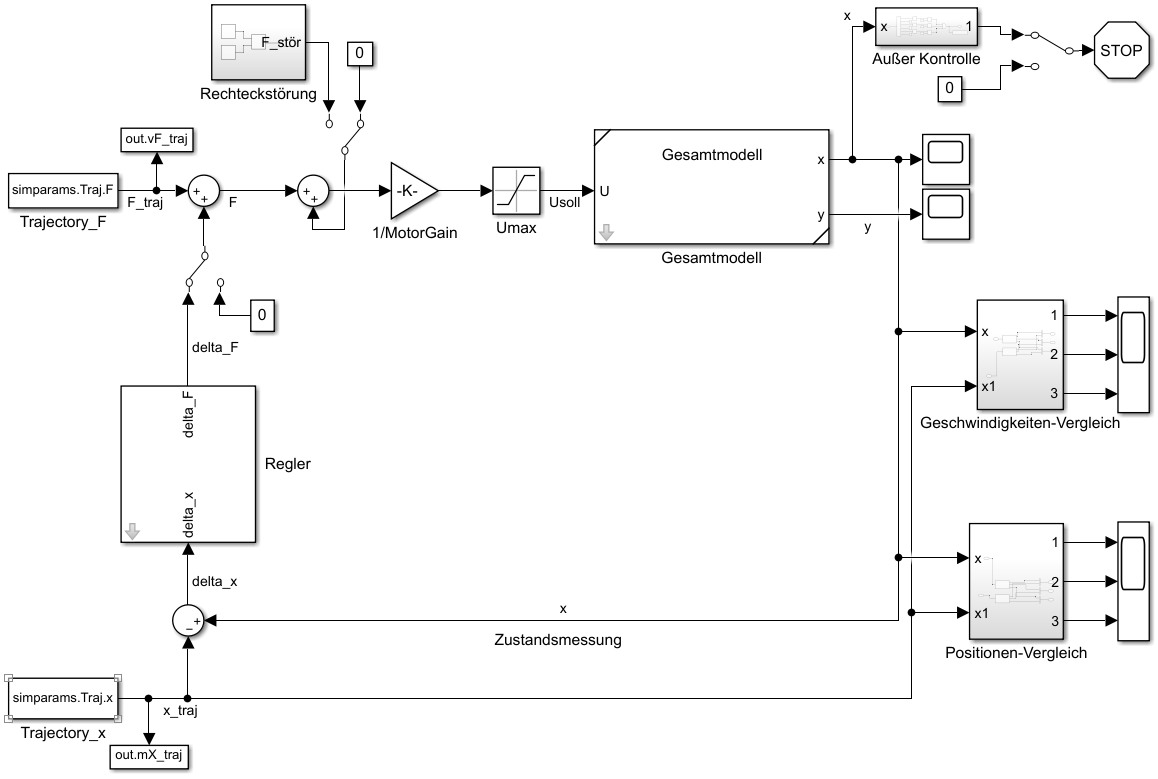
\includegraphics[width=0.98\textwidth]{Bilder/Simulink/TFR.PNG}
	\caption{Trajektorienfolgeregelung in Simulink}
	\label{fig:TFR_Simulink}
\end{figure}

Die Trajektorien werden der Simulation als \texttt{timeseries} mithilfe von \texttt{FromWorkspace} Blöcken zugeführt. Für die anschließende Auswertung in \Matlab\ hingegen können benötigte Signale über \texttt{ToWorkspace} an \Matlab\ gereicht werden. Um instabiles Verhalten zu erkennen und vorzeitig zu beenden, wird das Subsystem \texttt{AußerKontrolle} implementiert. Optional kann die Regelung zu Vergleichszwecken abgeschaltet werden. Ebenso kann kurzzeitig eine Rechteckstörung aufgeschaltet werden. Die genannten Optionen lassen sich über \texttt{ManualSwitches} ein- und ausschalten, wobei deren Zustand aus \Matlab\ heraus über die Funktion \texttt{set\_param} angesteuert werden kann.



%\section{Weitere Funktionen in \Matlab}
%...
%








\section{Stabilisierung der berechneten Trajektorien}\label{stabiltrj}

\newcommand{\scaleyplots}{0.6}

Für die mittels NMPC berechneten Trajektorien soll gezeigt werden, dass eine Stabilisierung in der Simulation mit Hilfe eines Trajektorienfolgereglers möglich ist. Im Rahmen der Vorgängerarbeit Fauvé \cite{fauve} war es nicht gelungen, die berechneten Trajektorien am störungsfreien System durch einen zeitvarianten Regler zu stabilisieren. Um das System zu stabilisieren, waren die Gewichtungsmatrizen \mat{Q} und $R$ für die Berechnung des Reglers variiert worden.

Aus diesem Grund wird ein anderer Ansatz gewählt, um eine Stabilisierung der mittels NMPC berechneten Trajektorien zu erreichen. Aus dem Skript \cite{modsim} zur Vorlesung \emph{Modellbildung und Simulation} ist bekannt, dass die Stabilität der Simulation maßgeblich von der Schrittweite und dem Integrationsverfahren abhängt. Bezüglich der Trajektorien können diese an zwei Stellen variiert werden: Einerseits innerhalb der NMPC zur Berechnung der Trajektorie und andererseits in der Simulation in \Simulink. Lässt sich eine Trajektorie mit verschiedenen Integrationsverfahren stabil simulieren, wird davon ausgegangen, dass das (ideale) System stabil ist. Über die Integration innerhalb der NMPC soll hingegen die Güte der berechneten Trajektorie variiert werden.


\subsection{Vorgehen}

Im Gegensatz zu den linearen Systemen können für nichtlineare Systeme nicht ohne Weiteres Stabilitätsgebiete für die verschiedenen Simulationsverfahren angegeben werden. Daher sind prinzipiell nur heuristische Ansätze anwendbar, um eine geeignete Schrittweite zu finden. Allgemein ist bei einer kleineren Schrittweite ein geringerer Schrittfehler und somit eine höhere Güte der Trajektorie zu erwarten. Andererseits steigen Rundungsfehler und Rechenzeit an. Bezüglich der Trajektorienberechnung wirkt sich besonders die Berechnungsdauer dominant aus. Bei einer kleineren Schrittweite muss darauf geachtet werden, dass der Prädiktionshorizont, der in Abtastpunkten angegeben wird, groß genug gewählt wird. Anderenfalls wird keine gültige Lösung mehr gefunden. Bei Fauvé \cite{fauve} wurde für die Trajektorienberechnung eine Schrittweite von $T=0,01$ (in Sekunden) bei einem Prädiktionshorizont von $N=350$ verwendet. Versuche zur Findung einer geeigneten Variation zu den von Fauvé \cite{fauve} verwendeten Parametern ergeben, dass $T=0.005$ und $N=500$ einen geeigneten Kompromiss aus möglichst kleiner Schrittweite und akzeptabler Rechenzeit liefern. 

Als Integrationsverfahren zur Trajektorienberechnung wurde von Fauvé \cite{fauve} das Euler-Verfahren eingesetzt. Als Alternative wird dem Euler-Verfahren nun das Runge-Kutta-Verfahren 4. Ordnung (RK4) gegenübergestellt.

Als weiterer Einflussfaktor auf die Güte der Trajektorien und somit auch auf ihre Stabilisierbarkeit werden die Systemparameter vermutet. Ihr Einfluss auf die Trajektorienberechnung wird in \secref{sec:trjparamtest} näher untersucht. Hierbei soll die Variation einzelner Systemparameter von einem Anfangs-Parametersatz ausgehen, für den sich die definierte Vergleichstrajektorie finden und stabilisieren lässt. Daher wird neben Schrittweite und Integrationsverfahren auch zwischen den in \secref{subsec:spdparams} definierten Parametersätzen \textit{Apprich} und \textit{Ribeiro} unterschieden.

Die Versuche zur Stabilisierbarkeit werden störungsfrei und unter Vernachlässigung der Coulomb-Reibung durchgeführt. Auf das Verhalten unter Berücksichtigung der Reibwerte wird in \secref{sec:trjparamtest} eingegangen. 

Um eine Vergleichbarkeit zur Vorgängerarbeit herzustellen, werden die Versuche sowohl mit als auch ohne Berücksichtigung der Gegeninduktion des Motormodells durchgeführt. 

Die Skripte \texttt{TFRSim\_SchlittenPendel\_run} und \texttt{TFRSim\_Gesamtmodell\_run} werden zur Durchführung der Simulationen implementiert. Beide Funktionen führen automatisiert drei Simulationen mit den Solvern \texttt{ode1} (Euler), \texttt{ode4} (RK4) und \texttt{ode45} (RK5(4) von Dormand-Prince) für eine mit \texttt{InitTrajReg} geladene Trajektorie durch. Darüber hinaus werden Plots und Animationen der Simulationsergebnisse erstellt. 
Bei den verwendeten Simulationsverfahren handelt es sich um explizite Einschrittverfahren. Der \texttt{ode4}-Solver (4. Ordnung) unterscheidet sich von \texttt{ode1} (1. Ordnung) im Wesentlichen durch die höhere Verfahrensordnung, wobei beide Verfahren mit konstanter Schrittweite operieren. Mit \texttt{ode45} wird zusätzlich ein Verfahren mit Schrittweitensteuerung eingesetzt. Hierbei handelt es sich wieder um ein Runge-Kutta-Verfahren, das jedoch gegenüber dem reinen RK4-Verfahren den Schrittfehler durch die Auswertung einer zusätzlichen Stützstelle schätzt und daraus für jeden Schritt eine eigene Schrittweite bestimmt.

Die Trajektorien werden für die Dauer des Prädiktionshorizonts und mit der gleichen Schrittweite, wie bei ihrer Berechnung verwendet wurde, simuliert. Ausnahme stellt \texttt{ode45} aufgrund der variablen Schrittweite da.

Die Funktion \texttt{TFRSim\_SchlittenPendel\_run} ruft das Simulinkmodell \texttt{TFR\_SchlittenPendel\_test} auf, das die Trajektorie direkt am Schlittenpendel-System simuliert, während \texttt{TFRSim\_Gesamtmodell\_run} das Simulinkmodell \texttt{TFR\_Gesamtmodell\_test} aufruft, das die Trajektorie am Gesamtsystem einschließlich des modellierten Gegeninduktionseffekts simuliert. Zum Vergleich werden die Trajektorien jeweils auch ohne Regler simuliert. Da die Simulationen störungsfrei sind, wird zunächst erwartet, dass auch eine Steuerung bereits gute Ergebnisse liefert.

Für die Berechnung des Reglers wurden im Voraus verschiedene QR-Matrizen als Ausgangskonfiguration getestet und sich schließlich für 
\[ 
	\mat{Q} = 
	\begin{bmatrix}
		1 & 0 & 0 & 0 & 0 & 0 \\
		0 & 1 & 0 & 0 & 0 & 0 \\
		0 & 0 & 1 & 0 & 0 & 0 \\
		0 & 0 & 0 & 1 & 0 & 0 \\
		0 & 0 & 0 & 0 & 1 & 0 \\
		0 & 0 & 0 & 0 & 0 & 1 \\
	\end{bmatrix} \ , \quad
	R = 0,1 \\
\]

entschieden, die der Arbeit von Chang \cite{chang} entnommen werden.


   

\subsection{Vergleichstrajektorie}\label{subsec:vglTrj}

Für die Versuche zur Stabilisierbarkeit und zum Einfluss der Systemparameter auf die Trajektorienberechnung (\secref{sec:trjparamtest}) wird eine Vergleichstrajektorie definiert.

Allgemein wird hierfür die klassische Aufschwungtrajektrie von AP1 nach AP4 gewählt. Es sind jedoch die in \secref{subsec:calctrj} vorgestellten Variationen zu beachten. Daher wird im Speziellen die Trajektorie 
\texttt{Traj14\_dev0\_-3.14\_-3.14\_x0max0.8} 
als Vergleichstrajektorie definiert. 
Anfangs- und Endzustand sind somit definiert als
\begin{align*}
	\vex_{\mrm{init}} =
	\begin{bmatrix}
		0 \\ 0 \\ -\pi \\ 0 \\ -\pi \\ 0
	\end{bmatrix}	, \qquad
	\vex_{\mrm{end}} =
	\begin{bmatrix}
		0 \\ 0 \\ 0 \\ 0 \\ 0 \\ 0
	\end{bmatrix} ,
\end{align*}


wobei die Positionsbeschränkung $-0,8 \leq x_0 \leq 0,8$ \ als Nebenbedingung fest vorgegeben wird.

Eine maximale Stellkraft wird in Abhängigkeit der Versuche zur Vergleichstrajektorie ergänzt.




\subsection{Ohne Gegeninduktion}\label{subsec:ohneInd}

Das System wird zunächst ohne die Gegeninduktion des Motormodells betrachtet, um im ersten Schritt an den Stand von Fauvé \cite{fauve} anzuknüpfen. Entsprechend wird auch die Stellkraftbegrenzung auf die in Fauvé \cite{fauve} verwendete Maximalkraft $F_{\mrm{max}}=\valunit{400}{N}$ eingestellt. 

Die Ergebnisse für $T=0.01$ und $N=350$ sind in \tabref{tab:T001N350Fmax400} zusammengefasst.
\begin{table}[h]
	\centering
	\caption{$T=0.01, \ N=350$}
		\begin{tabular}{c|c|c|c|c|c}
			\rowcolor[gray]{0.9}
			\multicolumn{2}{c|}{\textbf{Simulation}} & \multicolumn{2}{c|}{\textbf{Apprich}} & \multicolumn{2}{c}{\textbf{Ribeiro}} \\
			\midrule
			\rowcolor[gray]{0.9}
			\textbf{Solver} & \textbf{TFR} & \textbf{Euler} & \textbf{RK4} & \textbf{Euler} & \textbf{RK4} \\
			\midrule
			\cellcolor[gray]{0.9}  											& \cellcolor[gray]{.9}ohne & "`leicht instabil"' & instabil       & instabil & instabil\\
			\multirow{-2}{*}{\cellcolor[gray]{.9}ode1}	& \cellcolor[gray]{.9}mit  & \textbf{stabil} & \textbf{stabil} & instabil & "`leicht instabil"'\\
			\midrule
			\cellcolor[gray]{0.9}  											& \cellcolor[gray]{.9}ohne    & instabil	&  instabil & instabil & instabil\\
			\multirow{-2}{*}{\cellcolor[gray]{.9}ode4}	& \cellcolor[gray]{.9}mit     & instabil  & instabil  & instabil & \textbf{stabil}\\
			\midrule	
			\cellcolor[gray]{0.9}  											& \cellcolor[gray]{.9}ohne    & instabil &  instabil    & instabil 	& instabil\\
			\multirow{-2}{*}{\cellcolor[gray]{.9}ode45}	& \cellcolor[gray]{.9}mit     & instabil &  instabil    & instabil 	& "`leicht instabil"'\																							
		\end{tabular}
	\label{tab:T001N350Fmax400}
\end{table}

Es wird zwischen 

%\begin{center}
	%\begin{tabular}{cl}
		%stabil & Aufschwung gelingt, AP4 kann bis zum Ende der Simulation gehalten werden \\
		%"`leicht instabil"' & Aufschwung gelingt weitgehend, AP4 wird nicht gehalten  \\
		%instabil & Aufschwung gelingt nicht \\
	%\end{tabular}
%\end{center}
\begin{itemize}
	\item \emph{stabil} - Aufschwung gelingt, AP4 kann bis zum Ende der Simulation gehalten werden
	\item \emph{"`leicht instabil"'} - Aufschwung gelingt weitgehend, AP4 wird nicht gehalten
	\item \emph{instabil} - Aufschwung gelingt nicht
\end{itemize}
unterschieden. Zum besseren Verständnis soll die Zuordnung der dargestellten Ergebnisse an Hand repräsentativer Beispiele erläutert werden.

Zunächst wird der Eintrag links oben in \tabref{tab:T001N350Fmax400} betrachtet. Hierbei wird die Vergleichstrajektorie mit dem Apprich-Parametersatz und dem Euler-Verfahren berechnet und anschließend auch wieder mit dem Euler-Verfahren am Schlittendoppelpendel simuliert. Die in \figref{fig:F400T0.01_app_euler_ode1} dargestellten Ergebnisse zeigen die Verläufe der Ausgänge und der Stellkraft für das zunächst ungeregelte System. Es ist zu erkennen, dass der Aufschwung ohne Regelung gelingt, AP4 jedoch nicht gehalten wird. Das Ergebnis wird daher als \textit{leicht instabil} beurteilt. In der anschließenden Simulation am geregelten System kann das Pendel schließlich bis zum Ende der Simulationszeit stabilisiert werden.
\begin{figure}[h]
	\centering
		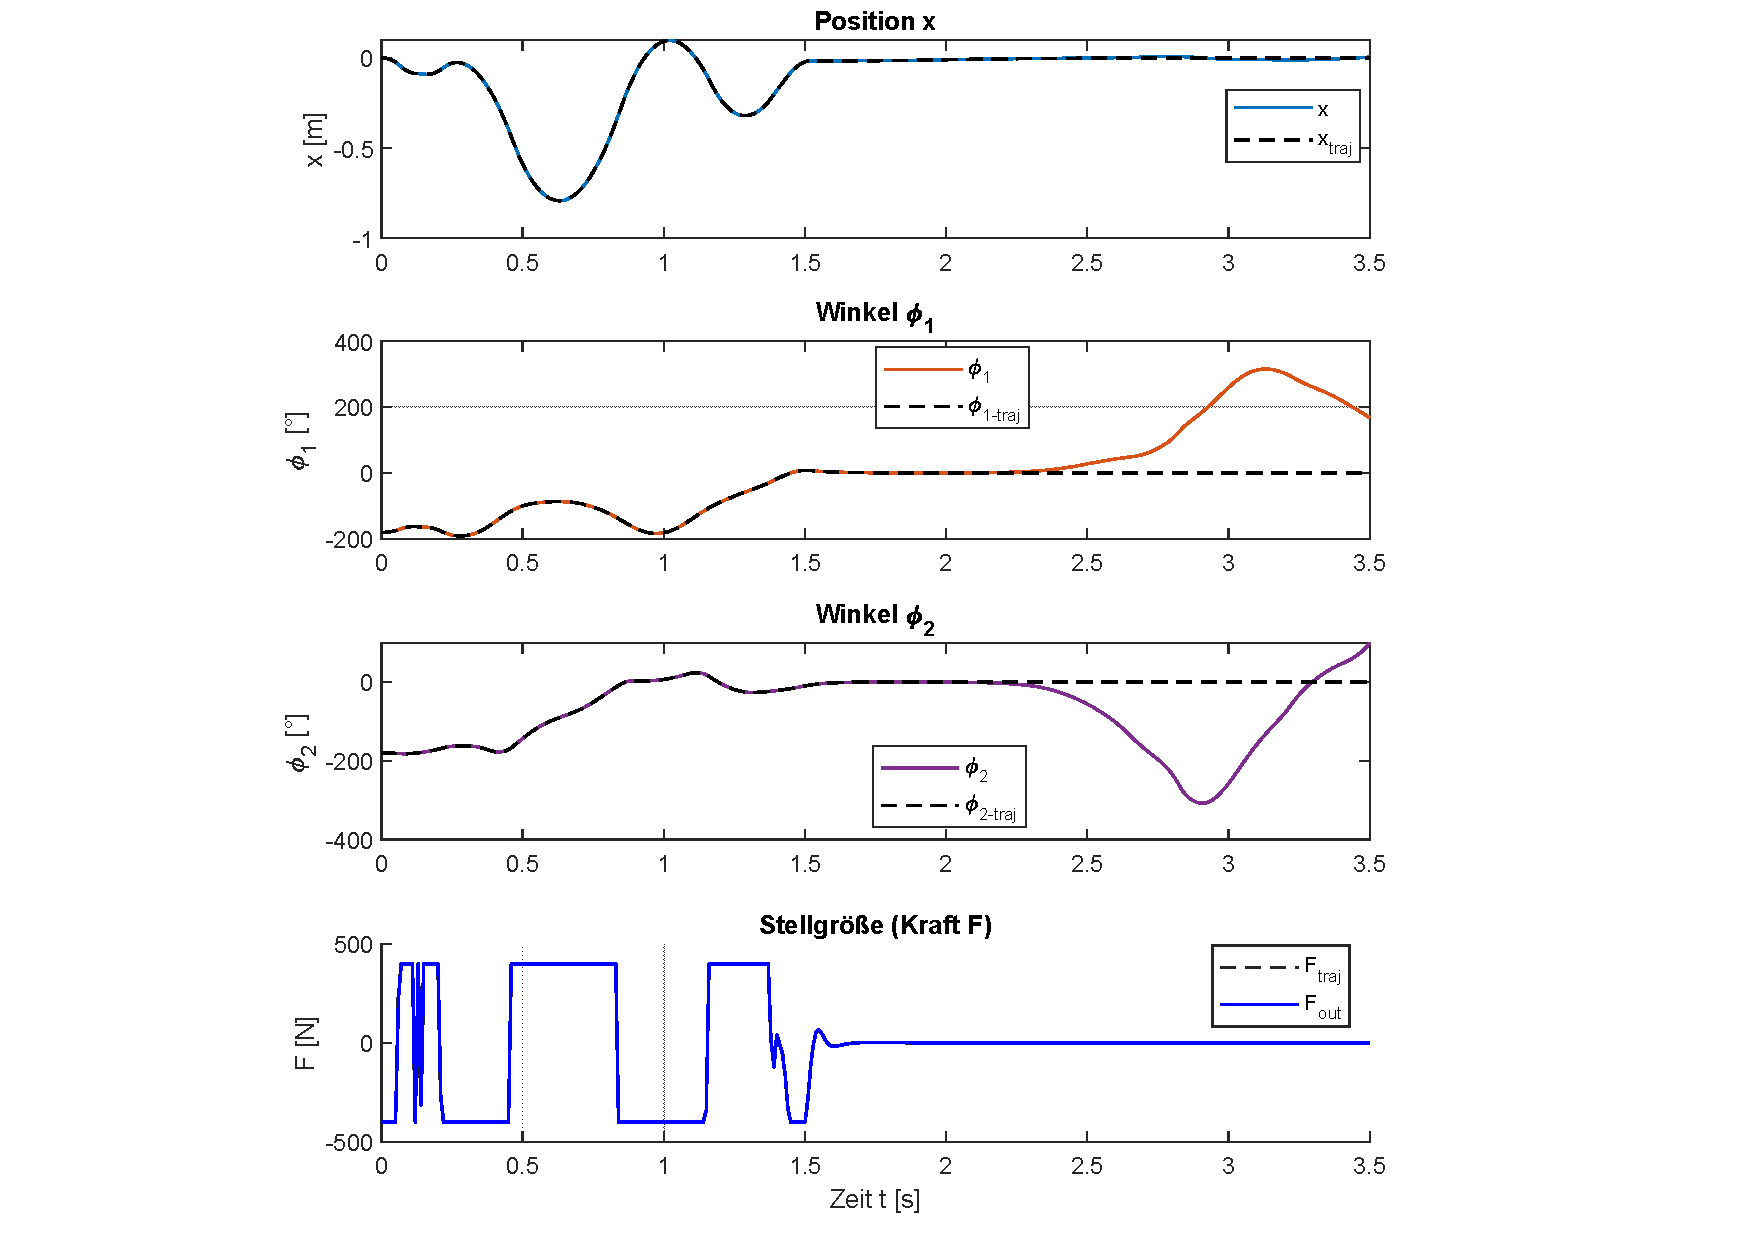
\includegraphics[scale=\scaleyplots]{Bilder/Trajektorien/F400T0.01_app_euler_ode1.pdf}
	\caption{$T=0,01$, $N=350$, Apprich-Parameter, Euler-MPC, ode1-Sim, ohne Regelung}
	\label{fig:F400T0.01_app_euler_ode1}
\end{figure}

Mit den Verfahren \texttt{ode4} und \texttt{ode45} am ungeregelten System zeigen die Verläufe demgegenüber hohe Abweichungen von der Trajektorie. Erwartungsgemäß lassen sie sich anschließend am geregelten System nicht stabilisieren. Die Verläufe werden daher als \textit{instabil} bewertet. 

Die mit dem Eulerverfahren berechnete Trajektorie lässt sich zwar stabilisieren, jedoch nur, wenn die bei der Trajektorienberechnung gemachten Schrittfehler durch das gleiche Verfahren in der Simulation näherungsweise reproduziert werden. Dass die Steuerung alleine nicht ausreicht, obwohl mit gleicher numerischer Fehlerfortpflanzung simuliert wird, lässt sich einerseits damit begründen, dass die Nebenbedingungen des Optimierungsverfahrens mit bestmöglicher, jedoch endlicher Genauigkeit eingehalten werden. Die beobachteten Genauigkeiten für die Nebenbedingungen liegen zwischen $10^{-13}$ und $10^{-34}$ für (lokal) optimale Lösungen. Andererseits ist insbesondere zu beachten, dass der zu erreichende Endwert durch die Optimierung lediglich angenähert wird. Die im Rahmen der Arbeit beobachteten absoluten Fehler einzelner Zustandsgrößen im letzten Prädiktionsschritt lagen bei den vom Optimierer ausgegebenen "`optimalen"' Lösungen im Bereich von $10^{-5}$ und $2 \cdot 10^{1}$.

Als weiteres Beispiel wird die für den Ribeiro-Parametersatz und das RK4-Verfahren berechnete Trajektorie in der Simulation mit \texttt{ode4} betrachtet. Die Verläufe sind für das ungeregelte System in \figref{fig:F400T0.01_rib_rk4_ode4} zu sehen. 
\begin{figure}[h]
	\centering
		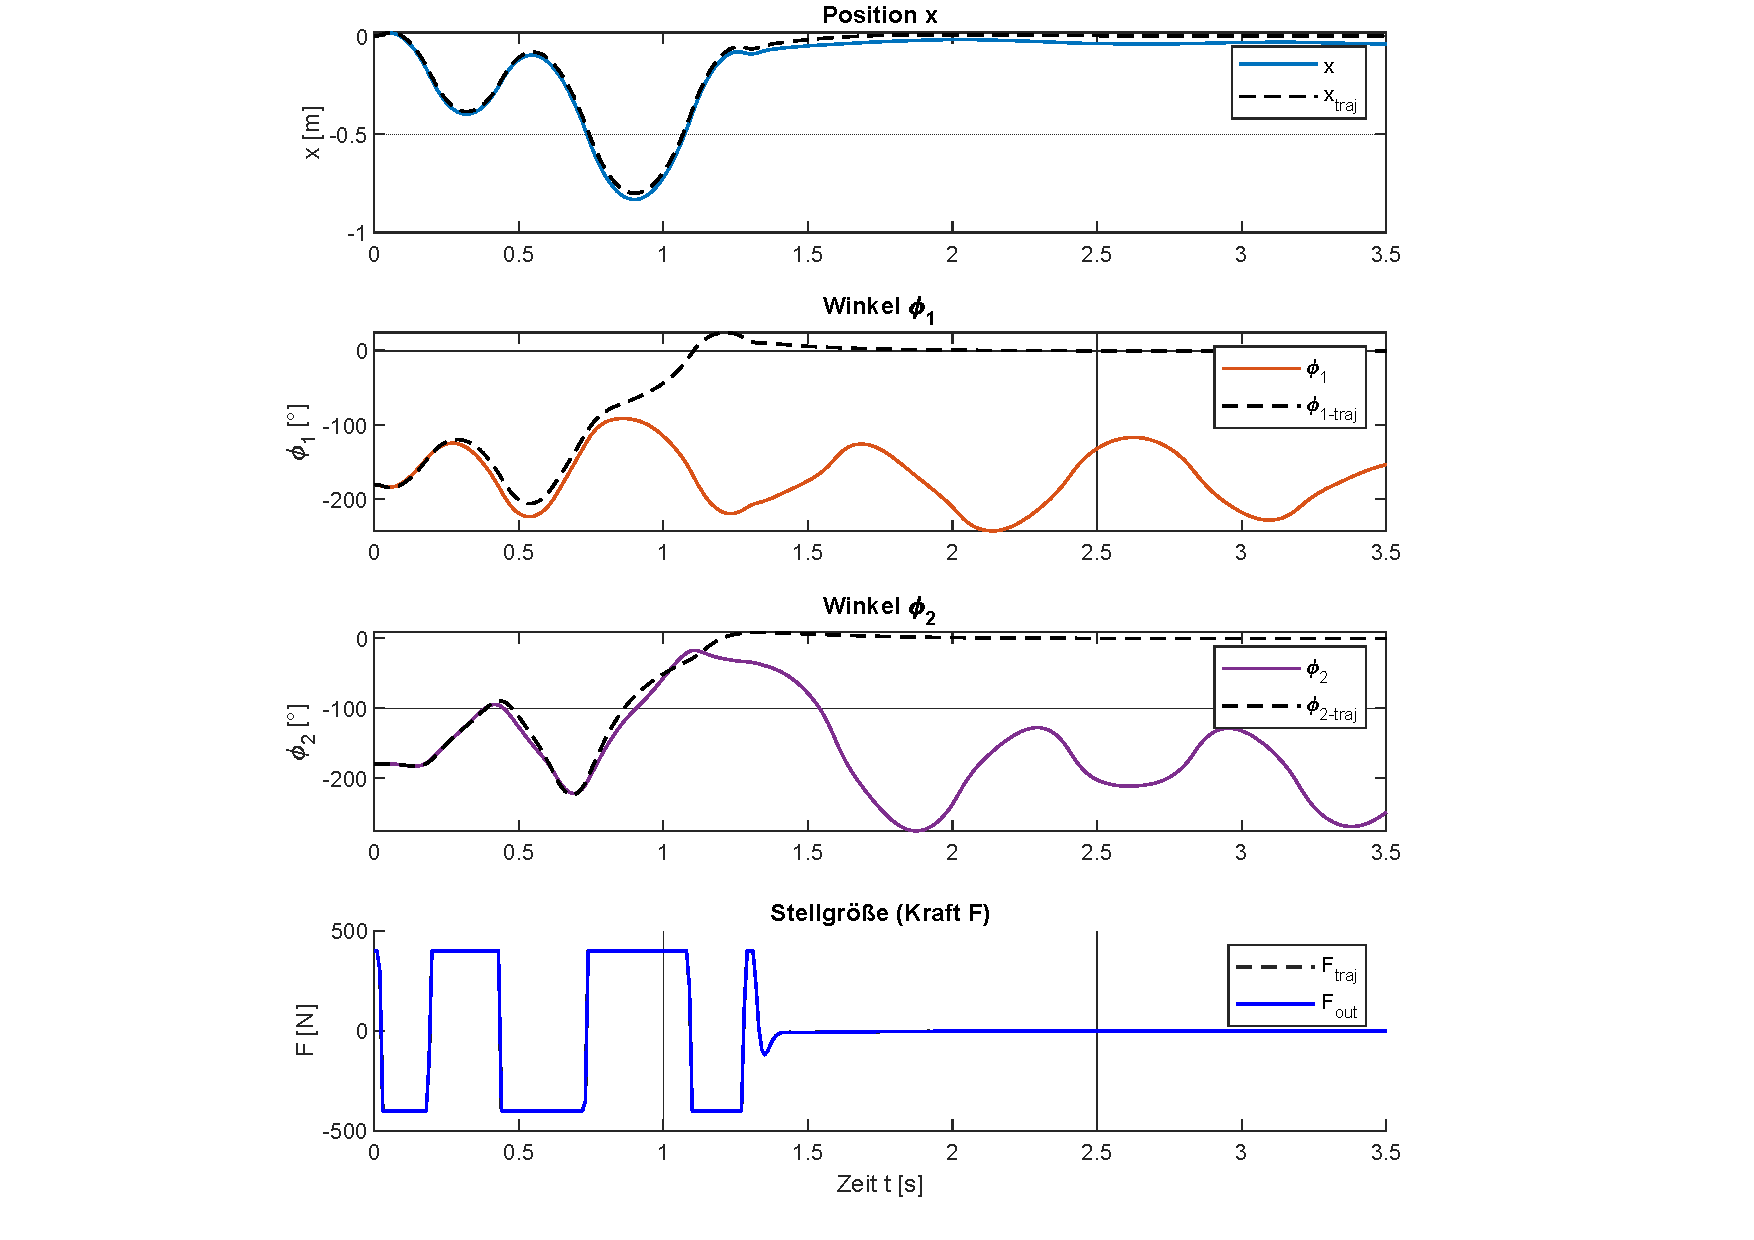
\includegraphics[scale=\scaleyplots]{Bilder/Trajektorien/F400T0.01_rib_rk4_ode4.pdf}
	\caption{$T=0,01$, $N=350$, Ribeiro-Parameter, RK4-MPC, ode4-Sim, ohne Regelung}
	\label{fig:F400T0.01_rib_rk4_ode4}
\end{figure}

Es ist deutlich ersichtlich, dass der Aufschwung nicht gelingt. Das erste Pendel fällt bereits gleich zu Anfang des Aufschwungs zurück, sodass in der Folge beide Pendel unkontrolliert zu schwingen beginnen. Die Verläufe werden daher als \textit{instabil} bewertet.
In \figref{fig:F400T0.01_rib_rk4_ode4_TFR_QR-alt} sind demgegenüber die Verläufe mit Trajektorienfolgeregelung zu sehen. 
\begin{figure}[h]
	\centering
		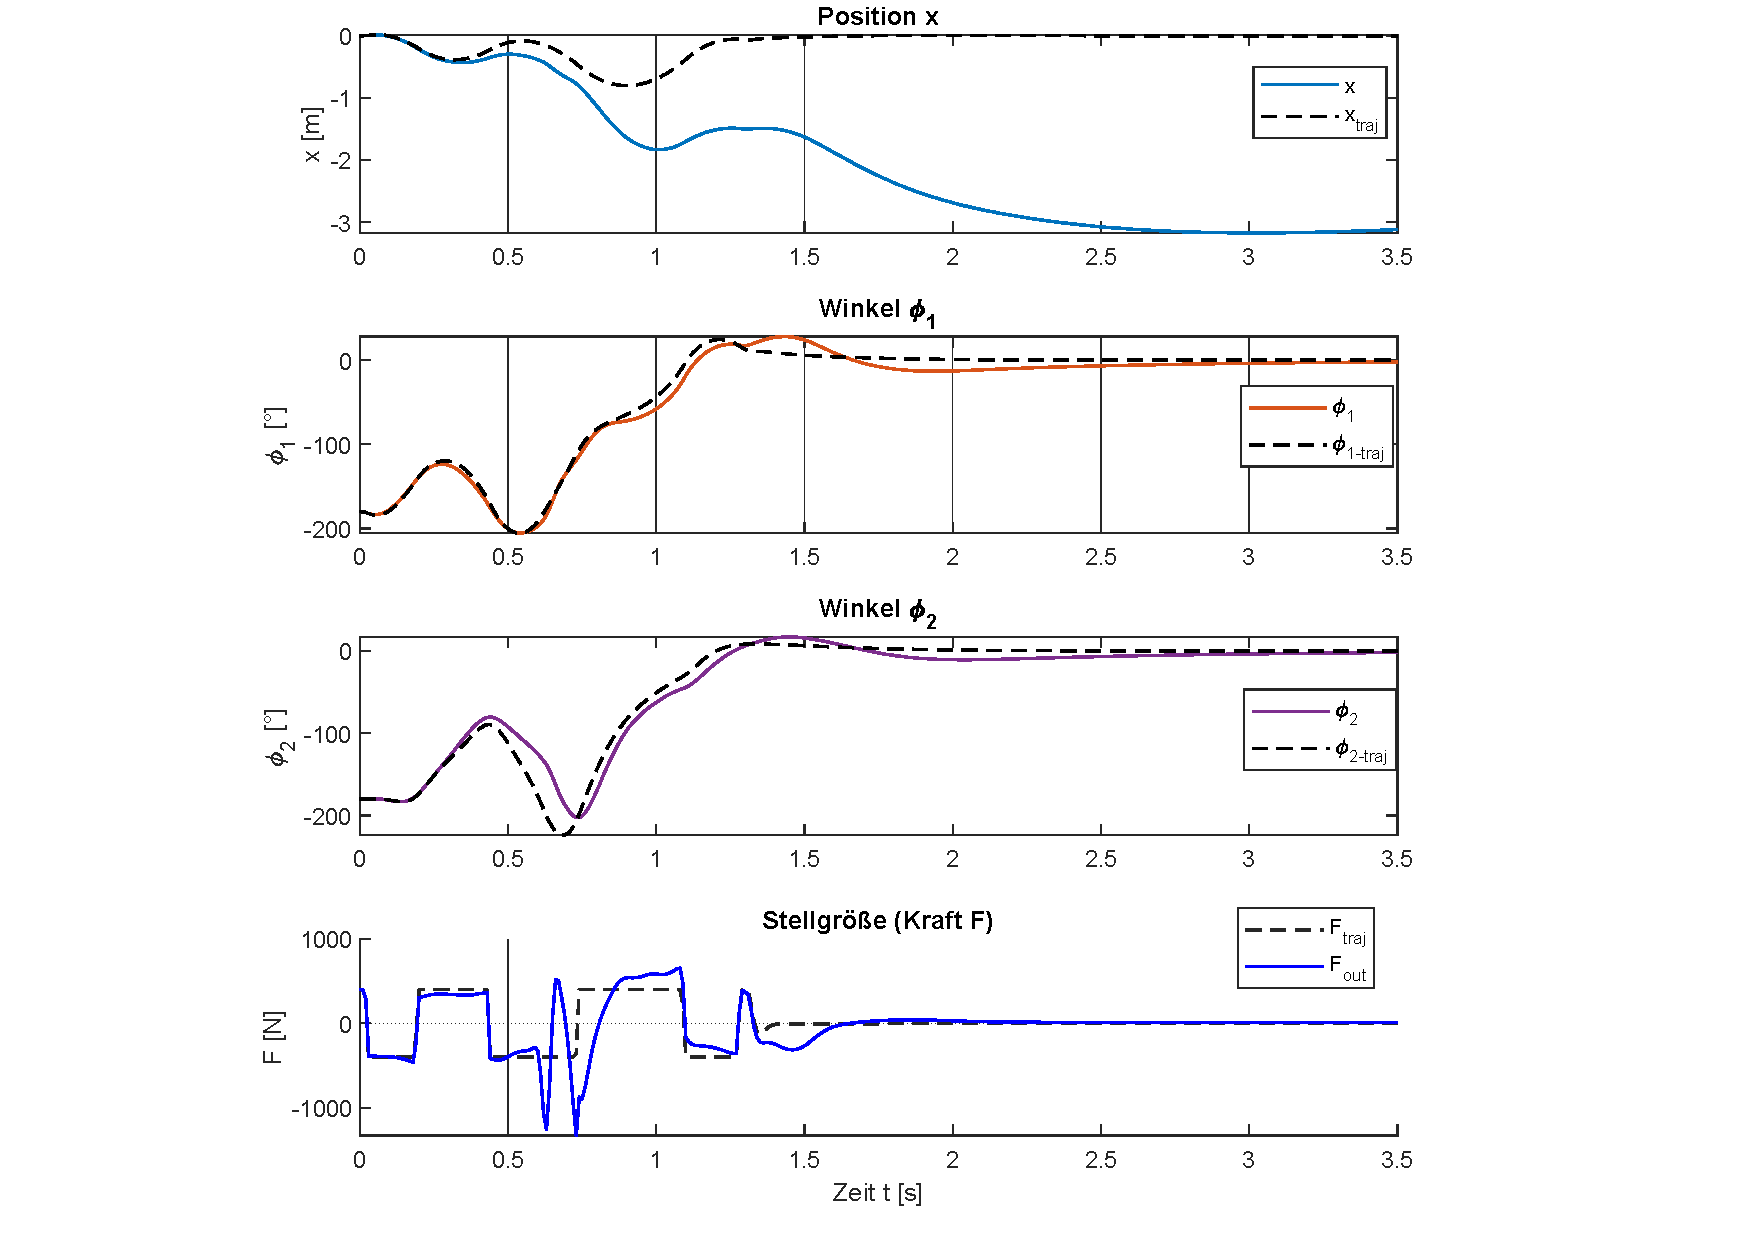
\includegraphics[scale=\scaleyplots]{Bilder/Trajektorien/F400T0.01_rib_rk4_ode4_TFR_QR-alt.pdf}
	\caption{$T=0,01$, $N=350$, Ribeiro-Parameter, RK4-MPC, ode4-Sim, mit Regelung}
	\label{fig:F400T0.01_rib_rk4_ode4_TFR_QR-alt}
\end{figure}

Das Doppelpendel kann demnach stabilisiert werden, jedoch ist in der Schlittenposition ein "`Weglaufen"' zu beobachten. Dieses sorgt dafür, dass die vorgegebene Positionsbegrenzung weit überschritten wird. Es liegt daher nahe, dass durch eine höhere Bestrafung der Position mit Hilfe der QR-Parameter des Reglers eine Verringerung der maximalen Auslenkung zu erwarten ist. Eine Variation von $Q_1$ ergibt, dass mit einer Erhöhung von $Q_1=1$ auf wahlweise $Q_1=1,05$ oder $Q_1=4,5$ sich die maximale Positionsauslenkung von etwa \valunit{-3,2}{m} auf \valunit{-2,5}{m} senken lässt. Damit liegt die erreichte Auslenkung weiterhin weit außerhalb der zulässigen Begrenzung von \valunit{\pm 0,8}{m}. Es zeigt sich außerdem, dass die Stabilisierung der betrachteten Trajektorie empfindlich auf Veränderung von $Q_1$ reagiert. Bereits bei $Q_1=1,07$ bzw. $Q_1=4,6$ wird das System instabil. Da allgemein jedoch eine Stabilisierung erreicht wird, ist die Trajektorie für die Simulation \texttt{ode4} am geregelten System als \textit{stabil} bewerten. 

Nach dem beschriebenen Vorgehen werden auch die weiteren Simulationsversuche ausgewertet. Die Ergebnisse in \tabref{tab:T001N350Fmax400} zeigen, dass sich drei der vier berechneten Trajektorien in zumindest einer der drei betrachteten Simulationen stabilisieren lässt. Die mit dem Euler-Verfahren und den Ribeiro-Parametern berechnete Trajektorie fällt dabei auf, da eine Stabilisierung generell in keiner der betrachteten Simulationen erreicht wird. Als Nächstes wird daher eine höhere Güte der Trajektorien gefordert, indem die Schrittweite für die Trajektorienberechnung halbiert wird bei entsprechender Erhöhung des Prädiktionshorizonts. Die Ergebnisse für $T=0.005$ und $N=500$ sind in \tabref{tab:T0005N500Fmax400} dargestellt.
\begin{table}[H]
	\centering
	\caption{$T=0.005, \ N=500$}
		\begin{tabular}{c|c|c|c|c|c}
			\rowcolor[gray]{0.9}
			\multicolumn{2}{c|}{\textbf{Simulation}} & \multicolumn{2}{c|}{\textbf{Apprich}} & \multicolumn{2}{c}{\textbf{Ribeiro}} \\
			\midrule
			\rowcolor[gray]{0.9}
			\textbf{Solver} & \textbf{TFR} & \textbf{Euler} & \textbf{RK4} & \textbf{Euler} & \textbf{RK4} \\
			\midrule
			\cellcolor[gray]{0.9}  											& \cellcolor[gray]{.9}ohne & "`leicht instabil"'  & "`leicht instabil"' & instabil & Trajektorie\\
			\multirow{-2}{*}{\cellcolor[gray]{.9}ode1}	& \cellcolor[gray]{.9}mit  & \textbf{stabil} & \textbf{stabil} 			& instabil 				 & 	\\
			\midrule
			\cellcolor[gray]{0.9}  											& \cellcolor[gray]{.9}ohne & instabil	& "`leicht instabil"' & instabil & nicht\\
			\multirow{-2}{*}{\cellcolor[gray]{.9}ode4}	& \cellcolor[gray]{.9}mit  & instabil & \textbf{stabil} & instabil & \\
			\midrule	
			\cellcolor[gray]{0.9}  											& \cellcolor[gray]{.9}ohne & instabil	&  "`leicht instabil"' & instabil 	& gefunden\\
			\multirow{-2}{*}{\cellcolor[gray]{.9}ode45}	& \cellcolor[gray]{.9}mit  & instabil	&  \textbf{stabil}  & instabil 	& \																											
		\end{tabular}
	\label{tab:T0005N500Fmax400}
\end{table}

Hierbei fällt auf, dass die Trajektorie, die mit Hilfe des Apprich-Parametersatzes und des RK4-Verfahrens berechnet wird, mit Hilfe des Reglers in allen drei Simulationen stabilisiert werden kann. Auch die Verläufe am ungeregelten System liefern bereits gute Ergebnisse. Die Stabilisierung durch den Regler erfolgt zudem innerhalb der vorgegebenen Positionsbegrenzung bei gleichzeitig geringer Abweichung von der Trajektorie.




\subsection{Mit Gegeninduktion}\label{subsec:mitInd}

Wird die Gegeninduktion des Motors berücksichtigt und am Gesamtmodell simuliert, fällt zunächst auf, dass mit $F_{\mrm{max}}= \valunit{400}{N}$ für den konstanten Bereich der Strombegrenzung keine der vier untersuchten Trajektorien gefunden wird. Durch eine Variation der Maximalkraftbegrenzung ergibt sich $F_{\mrm{max}}= \valunit{410}{N}$ als neue Grenze. Damit ist weiterhin eine Stellgrößenreserve von \valunit{11}{N} gegenüber der zuletzt am Versuchsstand eingestellten Maximalkraft von $F_{\mrm{max}}= \valunit{421}{N}$ gewährleistet. 

Für $T=0.01$ und $N=350$ kann dennoch keine der Trajektorien gefunden werden. Die Ergebnisse für $T=0.005$ und $N=500$ sind in \tabref{tab:T001N350Fmax410} zusammengetragen. Die Trajektorie auf Basis der Apprich-Parameter und des RK4-Verfahrens bestätigt die Ergebnisse aus \secref{subsec:ohneInd}. Sie lässt sich unabhängig vom betrachteten Simulationsverfahren stabilisieren.
\begin{table}[H]
	\centering
	\caption{$T=0.005, \ N=500$}
		\begin{tabular}{c|c|c|c|c|c}
			\rowcolor[gray]{0.9}
			\multicolumn{2}{c|}{\textbf{Simulation}} & \multicolumn{2}{c|}{\textbf{Apprich}} & \multicolumn{2}{c}{\textbf{Ribeiro}} \\
			\midrule
			\rowcolor[gray]{0.9}
			\textbf{Solver} & \textbf{TFR} & \textbf{Euler} & \textbf{RK4} & \textbf{Euler} & \textbf{RK4} \\
			\midrule
			\cellcolor[gray]{0.9}  											& \cellcolor[gray]{.9}ohne & Trajektorie  & instabil & leicht instabil & Trajektorie\\
			\multirow{-2}{*}{\cellcolor[gray]{.9}ode1}	& \cellcolor[gray]{.9}mit  &   						& \textbf{stabil} & \textbf{stabil} 				 & 	\\
			\midrule		
			\cellcolor[gray]{0.9}  											& \cellcolor[gray]{.9}ohne & nicht	& instabil 						& instabil & nicht\\
			\multirow{-2}{*}{\cellcolor[gray]{.9}ode4}	& \cellcolor[gray]{.9}mit  &        & \textbf{stabil}   	& instabil & \\
			\midrule	
			\cellcolor[gray]{0.9}  											& \cellcolor[gray]{.9}ohne & gefunden 	&  instabil    			& instabil 	& gefunden\\
			\multirow{-2}{*}{\cellcolor[gray]{.9}ode45}	& \cellcolor[gray]{.9}mit  &  					&  \textbf{stabil}  & instabil 	& \\																											
		\end{tabular}
	\label{tab:T001N350Fmax410}
\end{table}

Durch Variation der QR-Parameter können die Simulationsergebnisse zudem noch optimiert werden. Sehr gute Ergebnisse werden für die QR-Matrizen in \tabref{tab:NeueQR} erzielt.
\begin{table}[h]
	\centering
	\caption{Neue QR-Matrizen für Apprich-RK4-Trajektorie}
		\begin{tabular}{cll}
			\toprule
			ode1        & $\mat{Q} = \mrm{diag}\left(1, 1, 100, 1, 100, 1\right)$           & $R=0,01$ \\
			ode4, ode45 & $\mat{Q} = \mrm{diag}\left(1000, 0.01, 100, 0.1, 100, 0.1\right)$ & $R=0,001$ \\
			\bottomrule
		\end{tabular}
	\label{tab:NeueQR}
\end{table}

Die Ausgangsverläufe für die Simulation mit \texttt{ode45} und den neuen QR-Parametern sind in \figref{fig:F410T0.005_app_rk4_ode45_TFR_QR-neu} dargestellt. Im Vergleich zu den Plots in \secref{subsec:ohneInd} wird im Stellgrößenverlauf zusätzlich zwischen $F_\mrm{in}$ und $F_\mrm{out}$ unterschieden. $F_\mrm{in}$ bezeichnet den durch Regler und Trajektorie festgelegten Stellwert, der auf das Gesamtsystem gegeben wird. Auf Grund der Strombegrenzungskennlinie (vgl. \figref{fig:Stromkennlinie}) kann am Ausgang des Motors jedoch ein abweichender Kraftverlauf entstehen, der mit $F_\mrm{out}$ dargestellt wird. Da die Stromkennlinie in den Nebenbedingungen der Trajektorienberechnung berücksichtigt wird, entstehen Abweichungen zwischen $F_\mrm{in}$ und $F_\mrm{out}$ in erster Linie auf Grund des Reglers. 
\begin{figure}[h]
	\centering
		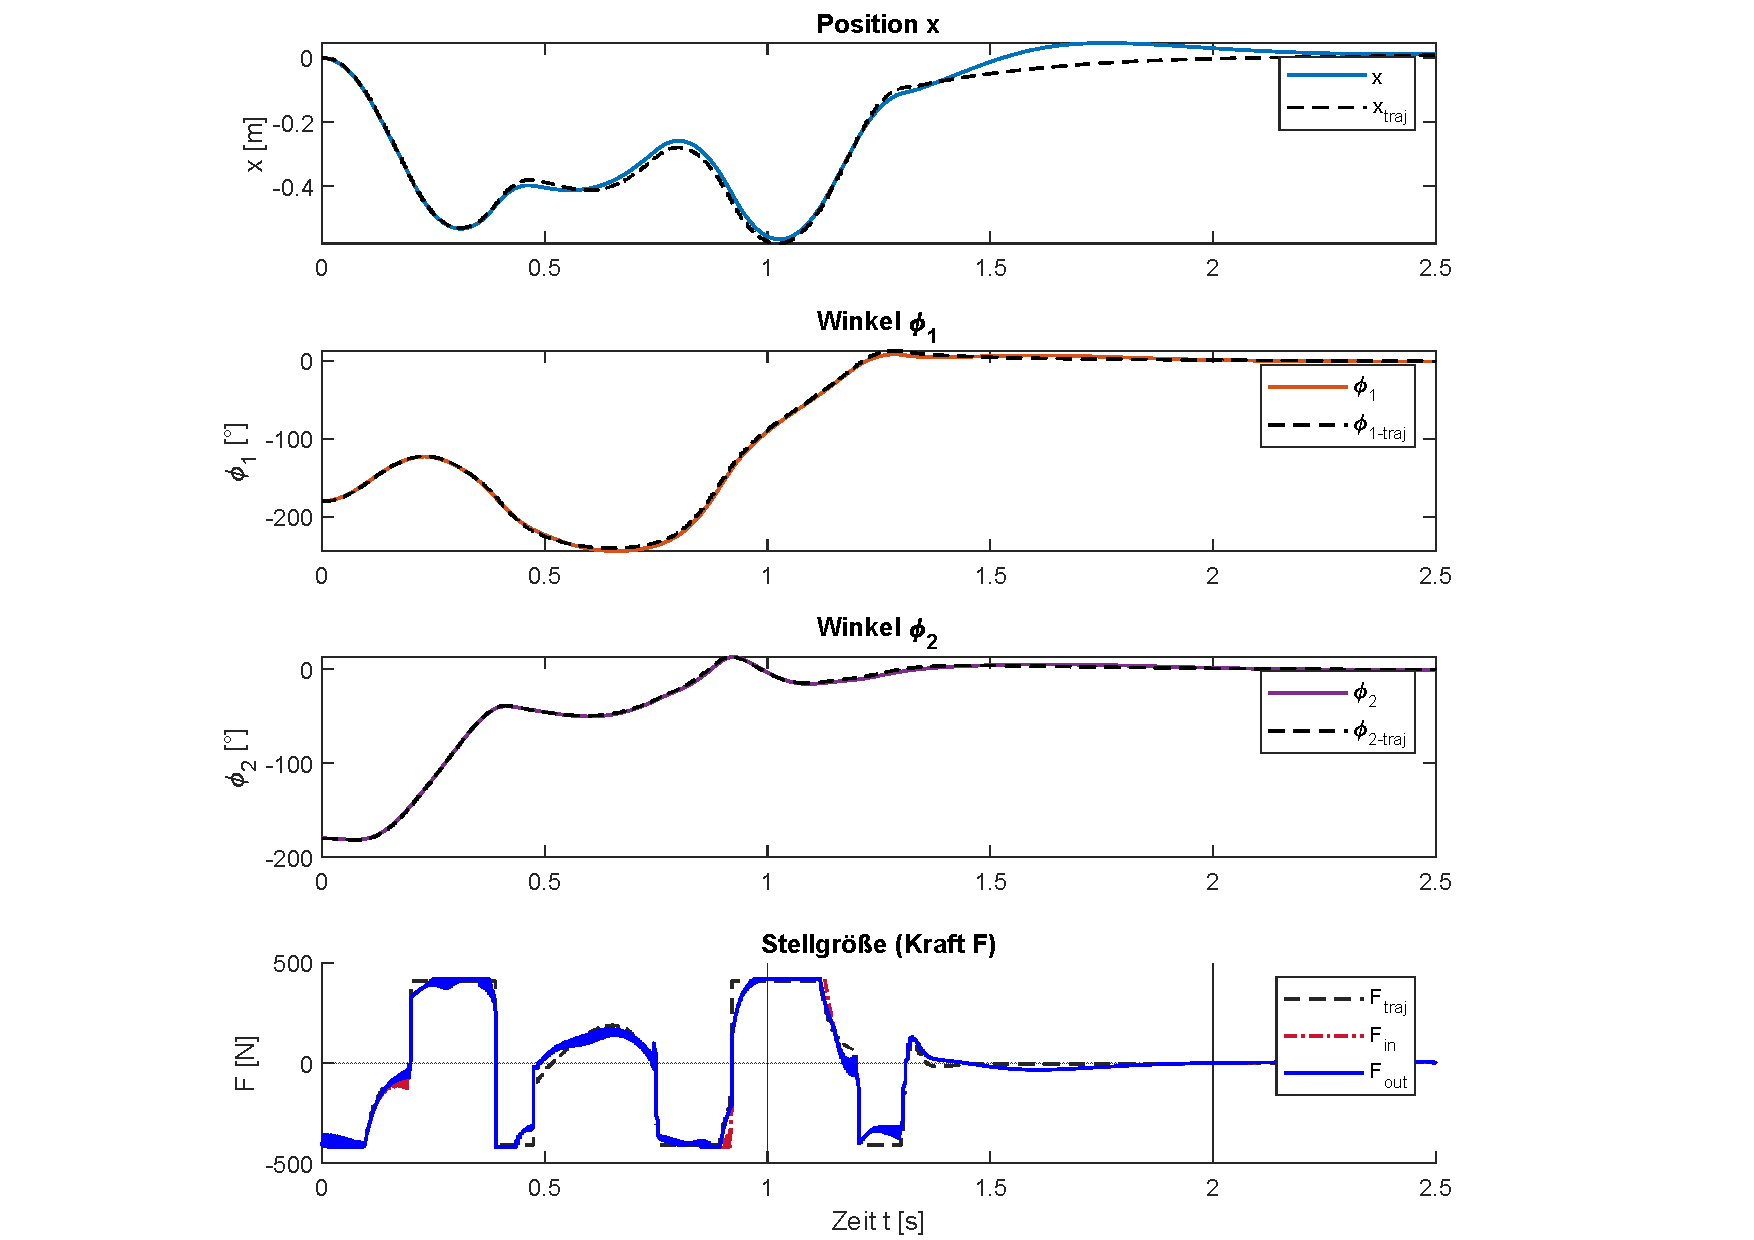
\includegraphics[scale=\scaleyplots]{Bilder/Trajektorien/F410T0.005_app_rk4_ode45_TFR_QR-neu.pdf}
	\caption{$T=0,005$, $N=500$, Apprich-Parameter, RK4-MPC, ode45-Sim, mit Regelung}
	\label{fig:F410T0.005_app_rk4_ode45_TFR_QR-neu}
\end{figure}

\textbf{Fazit:}
Es lässt sich zeigen, dass die mit dem Verfahren der NMPC berechneten Trajektorien in der Simulation stabilisierbar sind. Zudem bestätigt sich die Vermutung, dass die Schrittweite und die Wahl des Integrationsverfahrens zur Berechnung der Trajektorien einen Einfluss auf die numerische Stabilität haben. Eine geringere Schrittweite und ein Integrationsverfahren mit geringerem Schrittfehler haben in den betrachteten Versuchsdurchführungen zu einer höheren Stabilität geführt. Darüber hinaus fällt auf, dass die Apprich-Parameter gegenüber den Ribeiro-Parametern ein günstigeres Verhalten aufweisen. Der Einfluss der Modellparameter wird im folgenden Kapitel daher näher untersucht. 






\section{Untersuchung des Einflusses der Modellparameter}\label{sec:trjparamtest}

Im Folgenden soll der Einfluss der Modellparameter auf die Trajektorienberechnung untersucht werden.

\subsection{Vorgehen}

Gegenstand der Untersuchung sind die Parameter Masse, Massenträgheitsmoment und Schwerpunkt jedes Pendelstabs. Durch Variation der Parameter sollen günstige Wertebereiche identifiziert und formuliert werden, in denen gültige Trajektorien gefunden werden können. Darüber hinaus werden die Variationsergebnisse in Bezug auf Häufung und Güte der gültigen Trajektorien analysiert.

Die Parameterwerte für die Parameteruntersuchung orientieren sich an den Werten der zum Versuchsstand aufgestellten Parametersätze aus \secref{subsec:spdparams}. Die Schrittweiten der Parametervariationen werden möglichst gering gewählt, um die Aussagekraft der Ergebnisse durch eine hohe Auflösung sicherzustellen. Auf Grund der hohen Berechnungszeiten für die Trajektorien, sind beliebig kleine Schrittweiten jedoch nicht möglich, sodass ein sinnvoller Kompromiss zwischen Auflösung und Berechnungszeit gefunden werden muss. Das geplante Variationsvorhaben ist in \tabref{tab:Parametervariationen} aufgeführt. Hierbei wird die konstruktive Realisierbarkeit der Parameterwerte nicht berücksichtigt, da vorwiegend der Einfluss der Modellparameter auf die Berechnungsergebnisse untersucht wird.
\begin{table}[h]
	\centering
	\caption{Parametervariationen}
		\begin{tabular}{lllll}
	    \toprule
			Parameter & Startwert & Endwert & Schrittweite & Anzahl Trajektorien \\
			\midrule
			$m_1 \ [\unit{kg}]$     & $0$ & $2$    & $0,01$   & $201$ \\
			$m_2 \ [\unit{kg}]$     & $0$ & $2$    & $0,01$   & $201$ \\
			$J_1 \ [\unit{kgm^2}]$  & $0$ & $0,02$ & $0,0001$ & $201$ \\
			$J_2 \ [\unit{kgm^2}]$  & $0$ & $0,02$ & $0,0001$ & $201$ \\
		  $s_1 \ [\unit{m}]$      & $0$ & $0,29$ & $0,001$  & $291$ \\
			$s_2 \ [\unit{m}]$      & $0$ & $0,338$& $0,001$  & $339$ \\
			\bottomrule
		\end{tabular}
	\label{tab:Parametervariationen}
\end{table}

Die zu untersuchenden Modellparameter werden einzeln gegenüber einem definierten Ausgangsparametersatz variiert, wobei alle weiteren Parameter konstant gehalten werden. Zur Durchführung der Versuche wird die Funktion \texttt{examParameters} implementiert. Ihr kann eine Versuchsreihe bestehend aus der Bezeichnung des zu untersuchenden Parameters und einem Vektor mit den Variationswerten übergeben werden. Über den Aufruf der in \secref{subsec:searchtrj} beschriebenen Funktion \texttt{searchTrajectories} werden damit die benötigten Trajektorienberechnungen ausgeführt. Die Trajektorien werden anschließend im Ordner \texttt{ParameterExams} gespeichert. Um die Ergebnisse später sinnvoll identifizieren zu können, wird der in \secref{subsec:searchtrj} definierten Namenskonvention eine Endung bestehend aus der Bezeichnung des untersuchten Parameters und dessen Wert angefügt. 

Zur Bewertung der betrachteten Parametervariationen wird zunächst unterschieden, ob für die jeweilige Variation eine Trajektorie gefunden werden kann oder nicht. Darüber hinaus wird das Gütemaß $J_\mrm{dev}$ eingeführt, um die Güte der gefundenen Lösungen zu quantifizieren. Der Ansatz für das Gütemaß basiert auf der Definition von Trajektorien durch ihre Randbedingungen. Da diese bei der Optimierung mit endlicher Genauigkeit erfüllt werden (\vgl \secref{subsec:ohneInd}), ist der resultierende Fehler ein Kriterium für die Güte der Trajektorien.

Das Gütemaß wird mit
	\[
	J_\mrm{dev} = \left\| \Delta \ve{x_{\mrm{init}}} \right\| + \left\| \Delta \ve{x_{\mrm{end}}} \right\|
	\]
	
definiert. $\left\|\Delta \ve{x_\mrm{init}}\right\|$ und $\left\|\Delta \ve{x_\mrm{end}}\right\|$ sind hierbei als die euklidischen Normen der mit den Fehlerdifferenzen gefüllten Zustandsvektoren in Anfangs- und Endlage der Trajektorie zu verstehen.
\[
	\left\| \Delta \ve{x_{\mrm{init}}} \right\| = \sqrt{ \sum_{i=1}^6 \left( x_{\mrm{Traj,}i}(t_\mrm{init}) - x_{\mrm{init,}i} \right)^2 }
\]

mit $t_\mrm{init} = 0$ und
	\[
	\left\| \Delta \ve{x_{\mrm{end}}} \right\| = \sqrt{ \sum_{i=1}^6 \left( x_{\mrm{Traj,}i}(t_{\mrm{end}}) - x_{\mrm{end,}i} \right)^2 }
\]

mit $t_{\mrm{end}} = (N+1) \cdot T$

Wie in \secref{stabiltrj} erläutert, ist im Falle eine konvergierten Lösung nur der Endwertfehler relevant, da dieser indirekt durch die Zielfunktion und nicht durch die Nebenbedingungen für die Optimierung vorgegeben wird. Unter der Voraussetzung einer konvergierten Lösung gilt daher
\[
	J_\mrm{dev} = \left\| \Delta \ve{x_{\mrm{end}}} \right\| \ .
	\]	 

Basierend auf den Erkenntnissen des vorherigen Abschnitts wird weiterhin folgende Ausgangskonfiguration für die Berechnung der Trajektorien gewählt, wobei die Gegeninduktion des Motors berücksichtigt und die Coulomb-Reibung vernachlässigt wird:
\begin{itemize}
	\item $T = 0,005$
	\item $N = 500$
	\item RK4-Integration
	\item Apprich-Parameter
\end{itemize}

Als Trajektorie wird die in \secref{subsec:vglTrj} definierte Vergleichstrajektorie verwendet. Die Gewichtungsmatrizen für die Zielfunktion sind \secref{subsec:calctrj} zu entnehmen.






\subsection{Durchführung und Ergebnisse}\label{subsec:trjParTestRes}

Die Auswertung erfolgt mit Hilfe der Funktion \texttt{plot\_Jdev\_params}. Mit dieser wird das Gütemaß berechnet und über dem untersuchten Parameter in einem Koordinatensystem aufgetragen. Hierbei werden auch die berechneten Werte des Apprich- und des Ribeiro-Parametersatzes nach \secref{subsec:spdparams} als Vergleichswerte durch die Funktion hinzugefügt. Es ist zu beachten, dass der eingefügte Ribeiro-Vergleichswert sich nur auf den untersuchten Parameter bezieht. Die übrigen Parameter werden weiterhin dem Apprich-Parametersatz entnommen. Liegen die Werte von Apprich und Ribeiro nicht auf einem durch \tabref{tab:Parametervariationen} definierten Variationswert, ist eine Erhöhung der Anzahl an berechneten Trajektorien zu berücksichtigen. Trajektorien ohne lokale Konvergenz zu einem Optimum werden als ungültig gewertet.

Werden zunächst die relativen Häufigkeiten gültiger Trajektorien $\hg$ miteinander verglichen, zeigt sich, dass neben dem Massenträgheitsmoment von Stab 1 besonders die Variation der beiden Stabmassen einen vergleichsweise geringen Anteil an Trajektorien verzeichnet, bei denen der Optimierer lokal konvergiert \bzw eine gültige Lösung findet (\tabref{tab:statTrj}). Der Einfluss von $m_1$ und $m_2$ sowie $J_1$ auf die Trajektorienberechnung ist daher als hoch anzusehen. 

\begin{table}[h]
	\centering
	\caption{Statistik gültiger Trajektorien}
		\begin{tabular}{lllll}
			\toprule
			Parameter  & Ungültig & Gültig & Gesamt & Gültigkeitsanteil \hg \\
			\midrule
			$m_1 \ [\unit{kg}]$     & $177$ & $26$    & $203$   & $13 \% $ \\
			$m_2 \ [\unit{kg}]$     & $189$ & $14$    & $203$   & $7 \% $ \\
			$J_1 \ [\unit{kg m^2}]$  & $175$ & $28$    & $203$   & $14 \%$ \\
			$J_2 \ [\unit{kg m^2}]$  & $79$  & $124$   & $203$   & $61 \%$ \\
			$s_1 \ [\unit{m}]$      &  $231$  & $62$ & $293$  &  $21 \%$\\
			$s_2 \ [\unit{m}]$      & $190$ & $150$   & $340$  & $44 \%$ \\
			\bottomrule
		\end{tabular}
	\label{tab:statTrj}
\end{table}

Besonders auffällig ist in diesem Zusammenhang $m_2$ mit einem Anteil gültiger Trajektorien von nur $\hg=7\%$. \figref{fig:trjvarm2} visualisiert die Ergebnisse der $m_2$-Variation. Die Datenpunkte für Apprich und Ribeiro werden allgemein durch Quadrate markiert, wobei Dunkelblau für Apprich und Dunkelorange für Ribeiro steht. Da für die Ribeiro-Masse in diesem Fall keine gültige Trajektorie gefunden wird, erscheint der Wert als "`x"'-Markierung auf der Abszisse. Die übrigen ungültigen Trajektorien sind hingegen im Sinne der Übersichtlichkeit nicht explizit dargestellt.

\begin{figure}
	\centering
		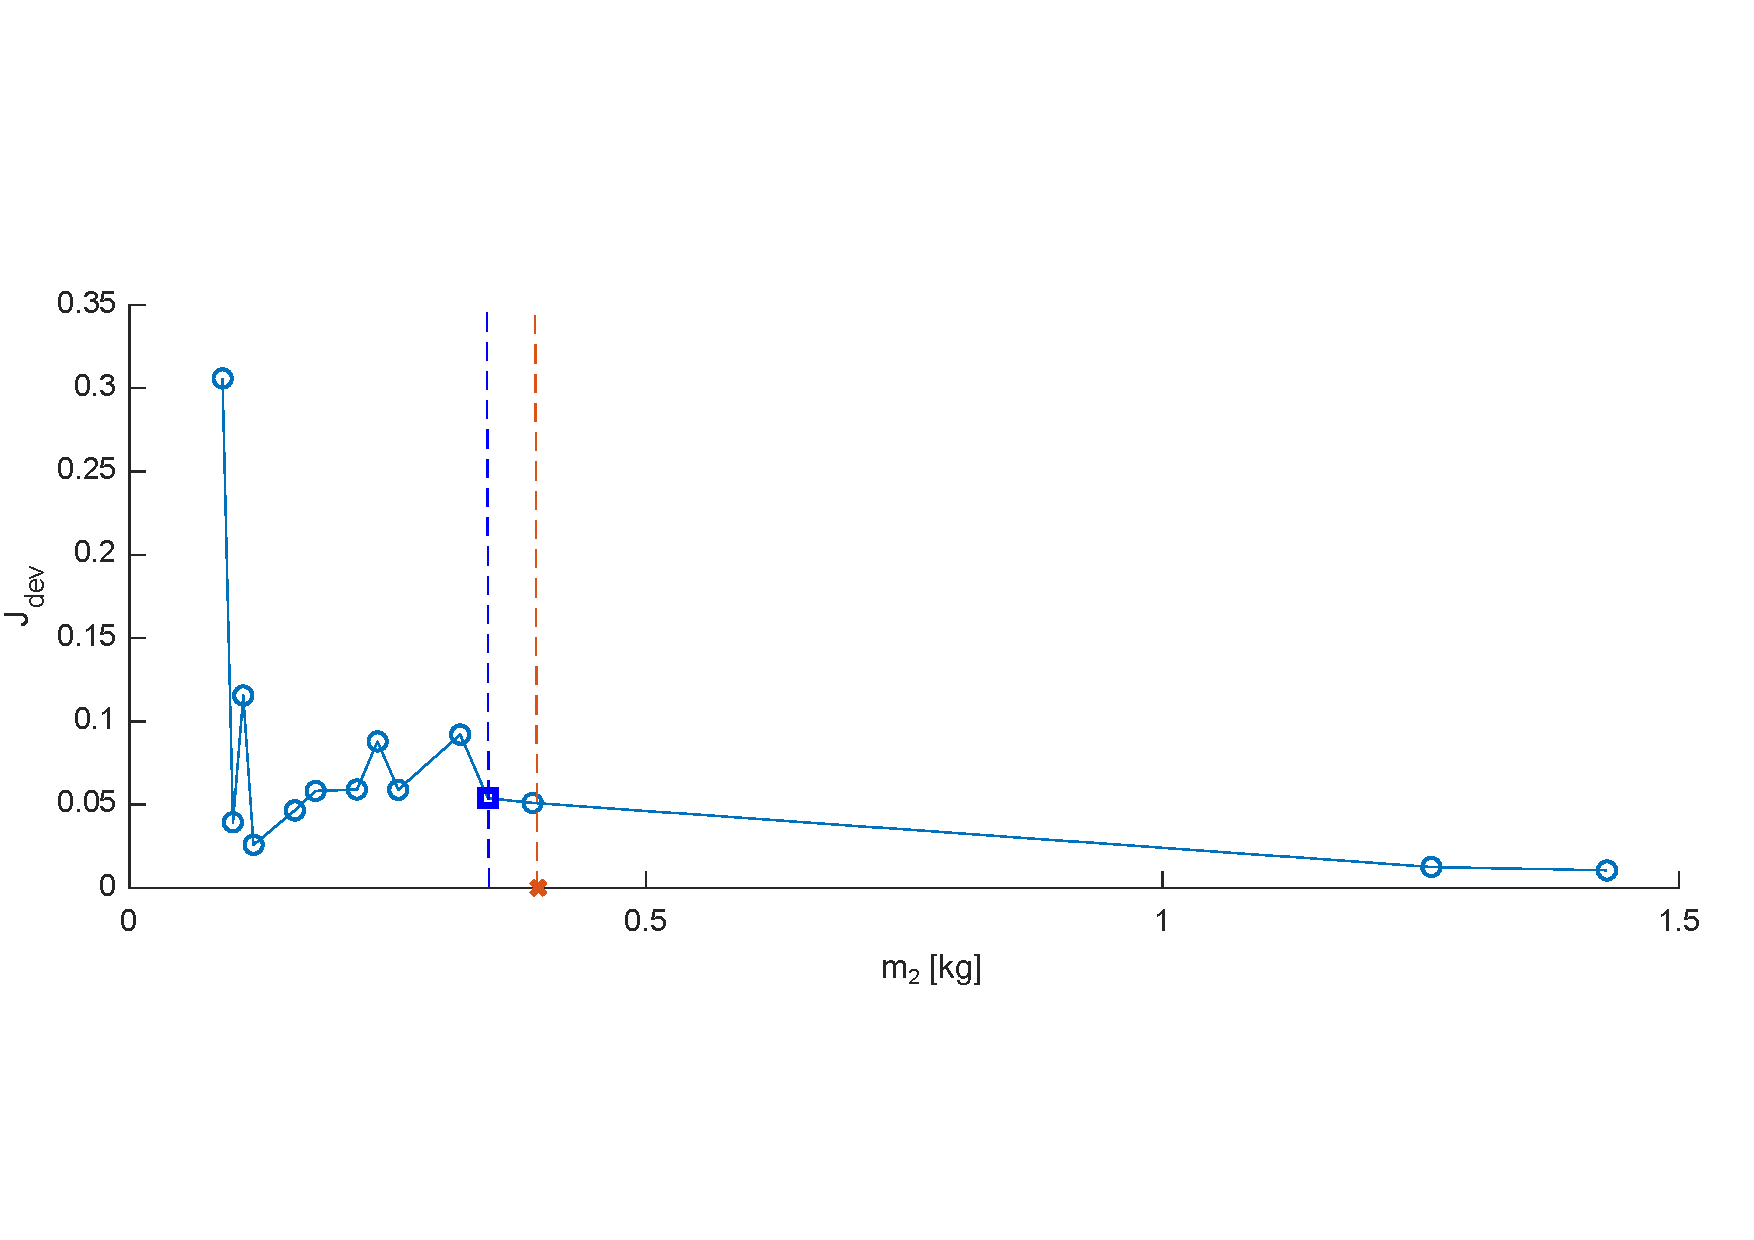
\includegraphics[width=0.8\textwidth]{Bilder/Trajektorien/m2.pdf}
	\caption{Variation $m_2$}
	\label{fig:trjvarm2}
\end{figure}

In der Abbildung zu erkennen ist, dass 12 von 14 gefundenen Trajektorien im Bereich $\valunit{0,09}{kg}\leq m_2 \leq\valunit{0,39}{kg}$ liegen. Zwei weitere Trajektorien werden gefunden, wenn der Wertebereich bis \valunit{1,43}{kg} deutlich vergrößert wird. Eine Erweiterung bis \valunit{2}{kg} führt schließlich zu keiner weiteren Trajektorie mehr. Wird nur der Bereich $\valunit{0,09}{kg}\leq m_2 \leq\valunit{0,39}{kg}$ betrachtet, steigt die Häufigkeit gültiger Trajektorien von $\hg=7\%$ auf $\hg=38\%$. Es treten jedoch weiterhin auch ungültige Lösungen auf. Zwischen den diskret untersuchten Parametern (vgl. \tabref{tab:Parametervariationen}) existieren im Kontinuierlichen unendlich viele weitere, potentielle Parameterwerte, für die eine Trajektorie berechnet werden kann. Wird die relative Häufigkeit gültiger Trajektorien $\hg$ als Konvergenz-Wahrscheinlichkeit  $\hg\approx\Pkon$ der Optimierung interpretiert, dann kann auch eine Aussage über die weiteren, potentiellen Trajektorien im Kontinuierlichen innerhalb des betrachteten Bereichs getroffen werden. Der Bereich $\valunit{0,09}{kg}\leq m_2 \leq\valunit{0,39}{kg}$ signalisiert somit allgemein eine hohe Konvergenzwahrscheinlichkeit $\Pkon$. Der markierte Apprich-Wert für $m_2$ befindet sich bereits nahe der Grenze dieses Bereichs, der Ribeiro-Wert sogar leicht darüber. Im Sinne einer hohen Konvergenzwahrscheinlichkeit kommt daher nur eine Verringerung von $m_2$ in Frage. 

Bei Betrachtung der Güte der gefundenen Trajektorien, fällt auf, dass für 12 von 14 Trajaktorien $J_\mrm{dev} = \left\| \Delta \ve{x_{\mrm{end}}} \right\|<0,1$ gilt. Besonders gut wird der Endwert für die beiden Trajektorien approximiert, die jedoch außerhalb des Bereichs von $\Pkon\approx38\%$ liegen und daher als "`Ausreißer"' bezeichnet werden. Die ungünstigeren Werte mit  $J_\mrm{dev}<0,1$ liegen hingegen im unteren Grenzbereich. Die Erfahrung in der Simulation hat gezeigt, dass für $J_\mrm{dev}\gg1$ ohne Weiteres keine QR-Matrizen für die Regelung gefunden werden, mit denen die Trajektorien stabilisiert werden können. Diese Trajektorien werden daher in Bezug auf Stabilisierbarkeit als ungünstig bis unbrauchbar eingeschätzt. Damit liegen die gefundenen Trajektorien mit $J_\mrm{dev}<1$ im akzeptablen Bereich. Ein eindeutiges Muster bezüglich der Trajektoriengüte lässt sich in \figref{fig:trjvarm2} jedoch nicht erkennen.

Für $m_2$ wird schließlich der Bereich $\valunit{0,09}{kg}\leq m_2 \leq\valunit{0,39}{kg}$ mit einer Konvergenzwahrscheinlichkeit von $\Pkon\approx\hg=38 \%$ als Wertebereich gültiger Trajektorien formuliert, wobei die zwei identifizierten "`Ausreißer"' vernachlässigt werden. Für den aktuelle Ribeiro-Parameter wird zudem empfohlen, diesen im Sinne des formulierten Wertebereichs zu verringern.

\begin{figure}
	\centering
		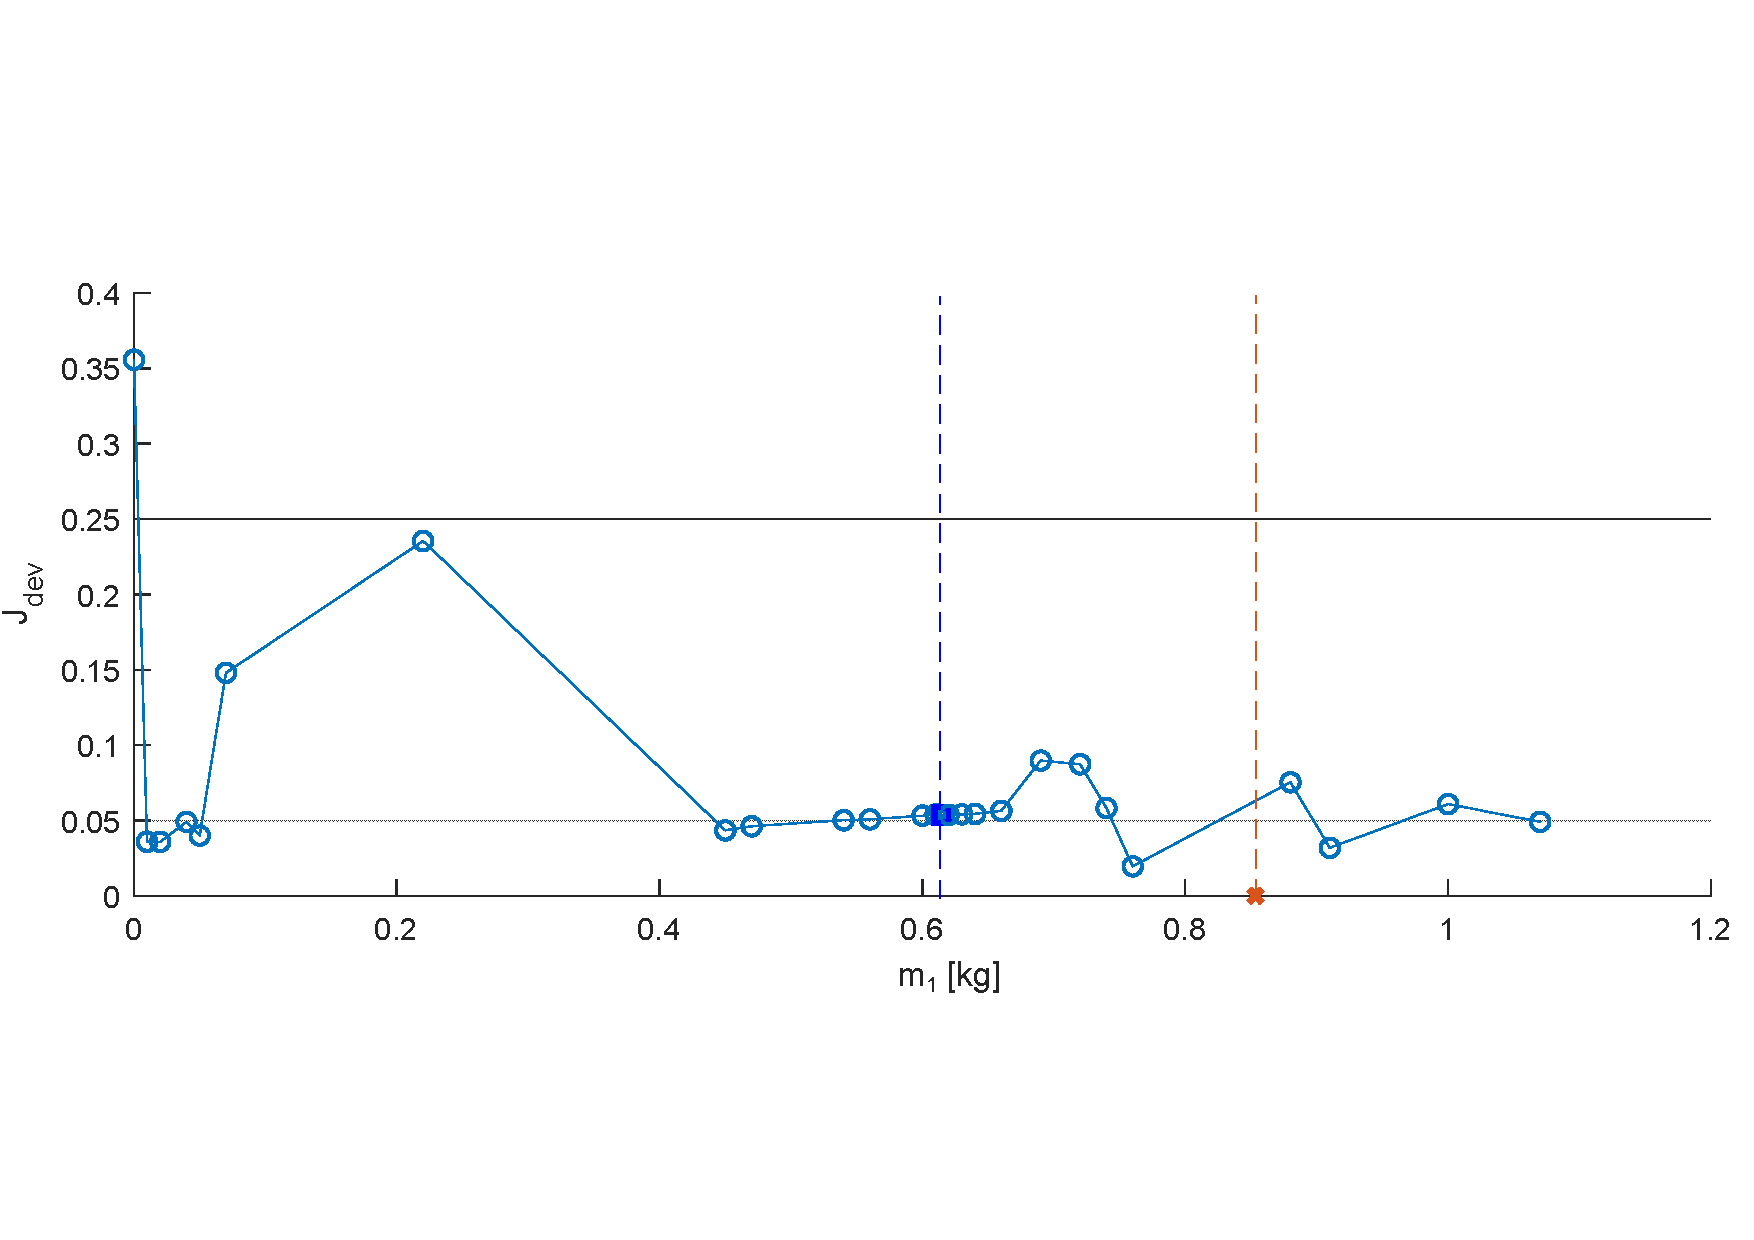
\includegraphics[width=0.8\textwidth]{Bilder/Trajektorien/m1.pdf}
	\caption{Variation $m_1$}
	\label{fig:trjvarm1} % etwas allgemein oder?
\end{figure}

Für $m_1$ lässt sich ein ähnliches Verhalten beobachten. Auch hier zeichnet sich der Bereich gültiger Trajektorien durch eine gut erkennbare Obergrenze ab. Diese liegt mit $m_{1\mrm{,max}}=\valunit{1,07}{kg}$ allerdings deutlich über der von $m_2$. Auffällig ist darüber hinaus eine Häufung gültiger Trajektorien mit hoher Güte im stark eingeschränkten Bereich $\valunit{0,6}{kg}\leq m_1 \leq\valunit{0,66}{kg}$ mit $\hg=88\%$, wo auch der Apprich-Wert einzuordnen ist. Bei einer Erweiterung des Bereichs auf $\valunit{0,45}{kg}\leq m_1 \leq\valunit{1,07}{kg}$ wird noch ein Anteil von $\hg=29\%$ erreicht. Eine ähnliche Häufung tritt im Bereich $\valunit{0}{kg}\leq m_1 \leq\valunit{0,07}{kg}$ mit $\hg=75\%$ auf, wobei die Bereichsgröße stark eingeschränkt ist. Allgemein liegen wie bei $m_2$ auch für $m_1$ die Trajektorien mit einer geringeren Güte von $J_\mrm{dev}<0,1$ im unteren Bereich. Besonders ungünstige Trajektorien mit $J_\mrm{dev}\gg1$ treten allerdings erneut nicht auf. Auch wird wieder für den Ribeiro-Parameter keine Lösung gefunden, wobei dieser nun in einem Bereich liegt, in dem prinzipiell Lösungen gefunden werden.

Allgemein wird als Wertebereich $\valunit{0}{kg}\leq m_1 \leq\valunit{1,07}{kg}$ formuliert, wobei $\Pkon\approx\hg=26 \%$ gilt. 

Anders als bei den Massen unterscheiden sich die Massenträgheitsmomente in ihrem Verhalten recht deutlich. Während für $J_1$ bezogen auf die Anzahl untersuchter Werte nur ein Anteil gültiger Trajektorien von $14 \%$ vorliegt, werden für $J_2$ mit einem Anteil von $61\%$ überwiegend gültige Trajektorien gefunden. Dies deutet auf einen geringen Einfluss von $J_2$ auf die Trajektorienberechnung hin. Die in \figref{fig:trjvarJ2} dargestellten Ergebnisse zeigen, dass beinahe über den gesamten Variationsraum von $J_2$ Trajektorien gefunden werden. Lediglich im untersten Bereich $\valunit{0}{kg m^2}\leq J_2 < \valunit{0,004}{kg m^2}$ können keine Trajektorien gefunden werden. In diesem Bereich ist der Ribeiro-Parameter angesiedelt, für den entsprechend keine Trajektorie gefunden wird. Der Apprich-Parameter befindet sich mit \valunit{0,00407}{kg m^2} unmittelbar im Grenzbereich. Durch eine Untergrenze der Wertebereichs mit $\valunit{0,004}{kg m^2}\leq J_2 \leq \valunit{0,02}{kg m^2}$ liegt der Anteil gültiger Trajektorien bei $77\%$. Wird die Untergrenze auf $J_{2\mrm{min}} = \valunit{0,0152}{kg m^2}$ erhöht, ergeben sich mit $\hg=100 \%$ ausschließlich gültige Trajektorien über den gesamten Bereich. Die Trajektoriengüte unterliegt im Bereich von $\hg=100 \%$ jedoch starken Schwankungen

\begin{figure}
	\centering
		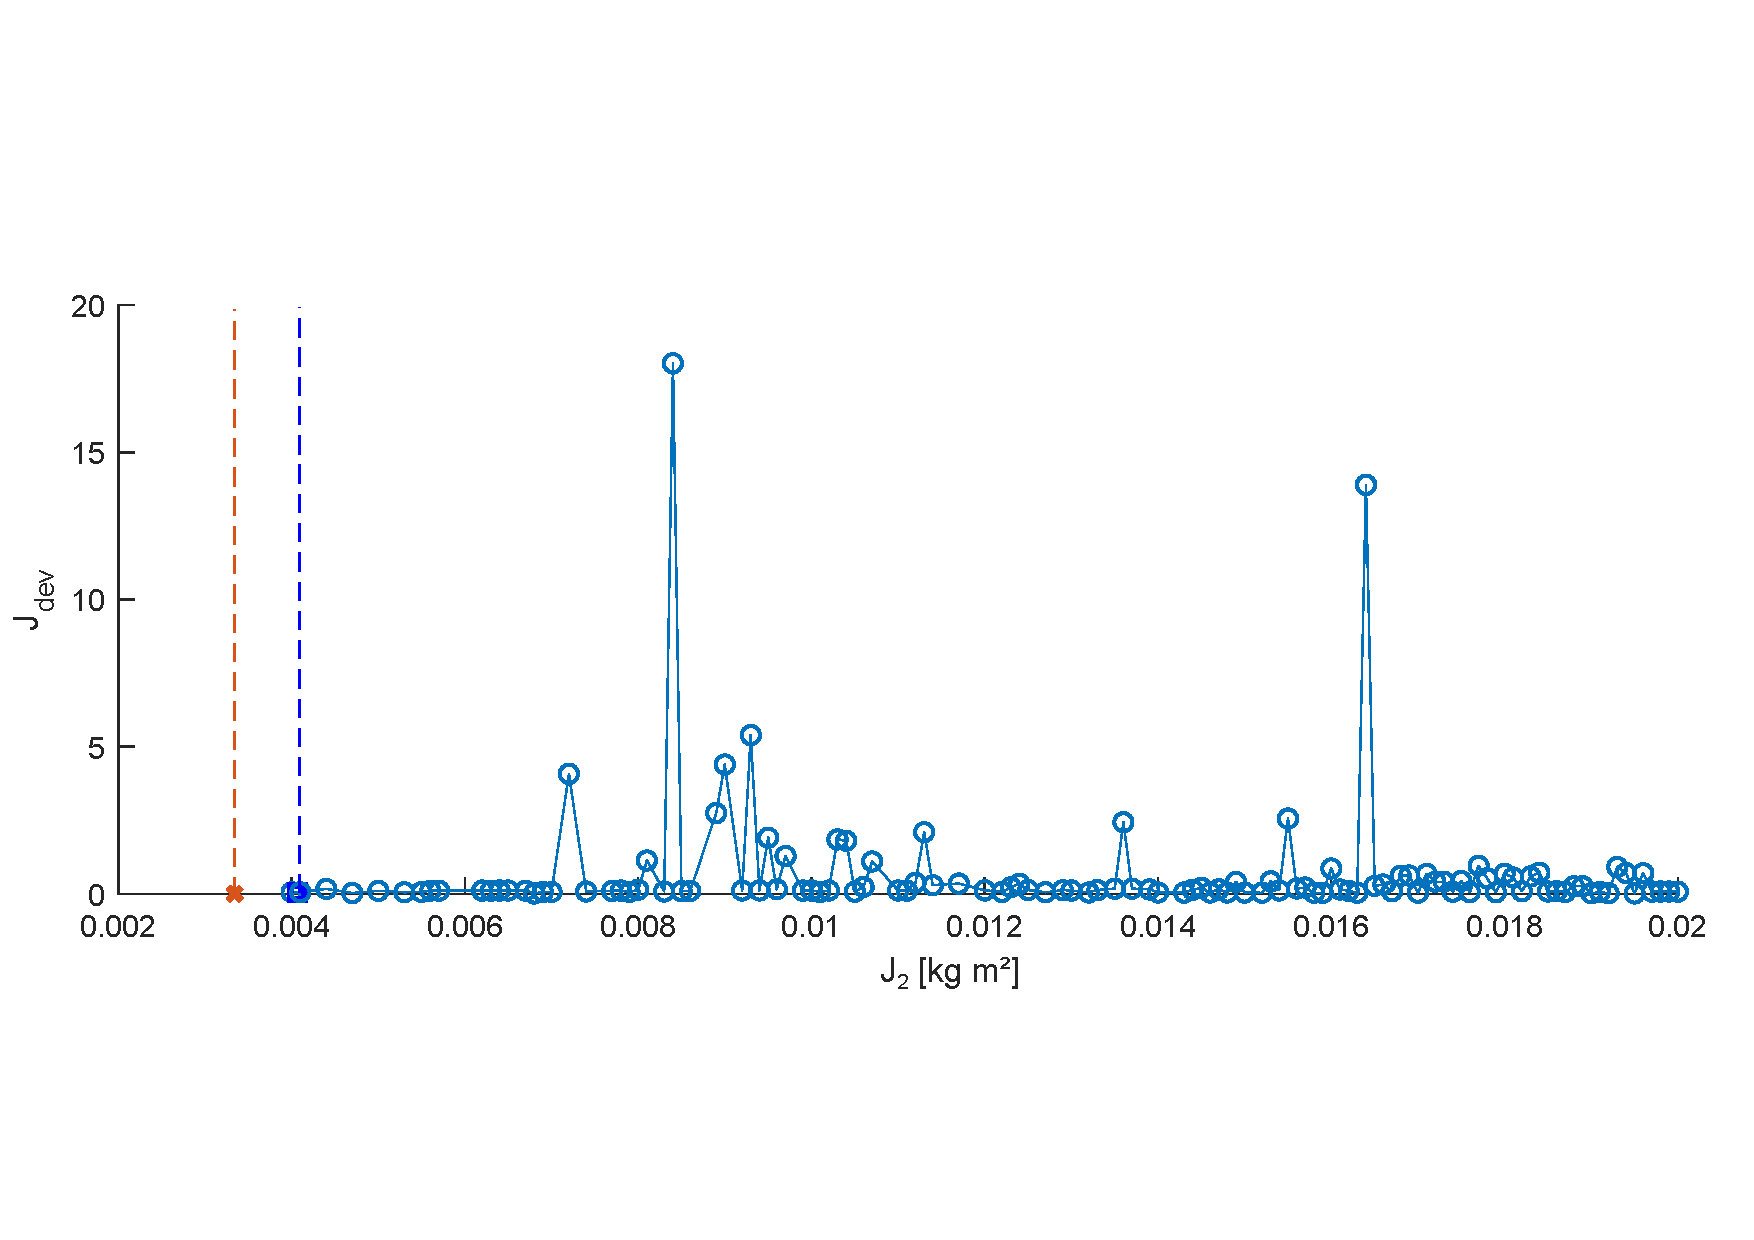
\includegraphics[width=0.8\textwidth]{Bilder/Trajektorien/J2.pdf}
	\caption{Variation $J_2$}
	\label{fig:trjvarJ2}
\end{figure}

Anders als bei den Stabmassen treten für $J_2$ erstmals besonders hohe Werte der Gütefunktion von $J_\mrm{dev}>>1$. Die für $J_2=\valunit{0,0084}{kg m^2}$ gefundene Trajektorie erreicht einen Wert von $J_\mrm{dev}=18,02$ und ist damit als unbrauchbar anzusehen. Im Bereich $\valunit{0,0072}{kg m^2}\leq J_2 \leq \valunit{0,0113}{kg m^2}$ tritt eine leichte Häufung von Trajektorien mit hohem $J_\mrm{dev}$ auf. Da es sich dennoch um lokale Minima und somit aus Sicht des Optimierers um gültige Trajektorien handelt, entsteht der hohe Wert weiterhin alleine aufgrund der hohen Ungenauigkeit der Approximation der Endlage. Für die weitere Verwendung berechneter Trajektorien ist daher dringend die Approximationsgüte zu überprüfen. Auch im beschriebenen Bereich von $\hg=100 \%$ treten vereinzelt gültige Trajektorien sehr geringer Güte auf.

Als Wertebereich gültiger Lösungen wird der Bereich $\valunit{0,004}{kg m^2}\leq J_2 \leq \valunit{0,02}{kg m^2}$ mit $\Pkon\approx\hg=77 \%$formuliert. Es wird zudem eine Erhöhung des aktuellen Ribeiro-Werts für $J_2$ empfohlen, sodass sich dieser zukünftig innerhalb des empfohlenen Wertebereichs befindet.

\begin{figure}
	\centering
		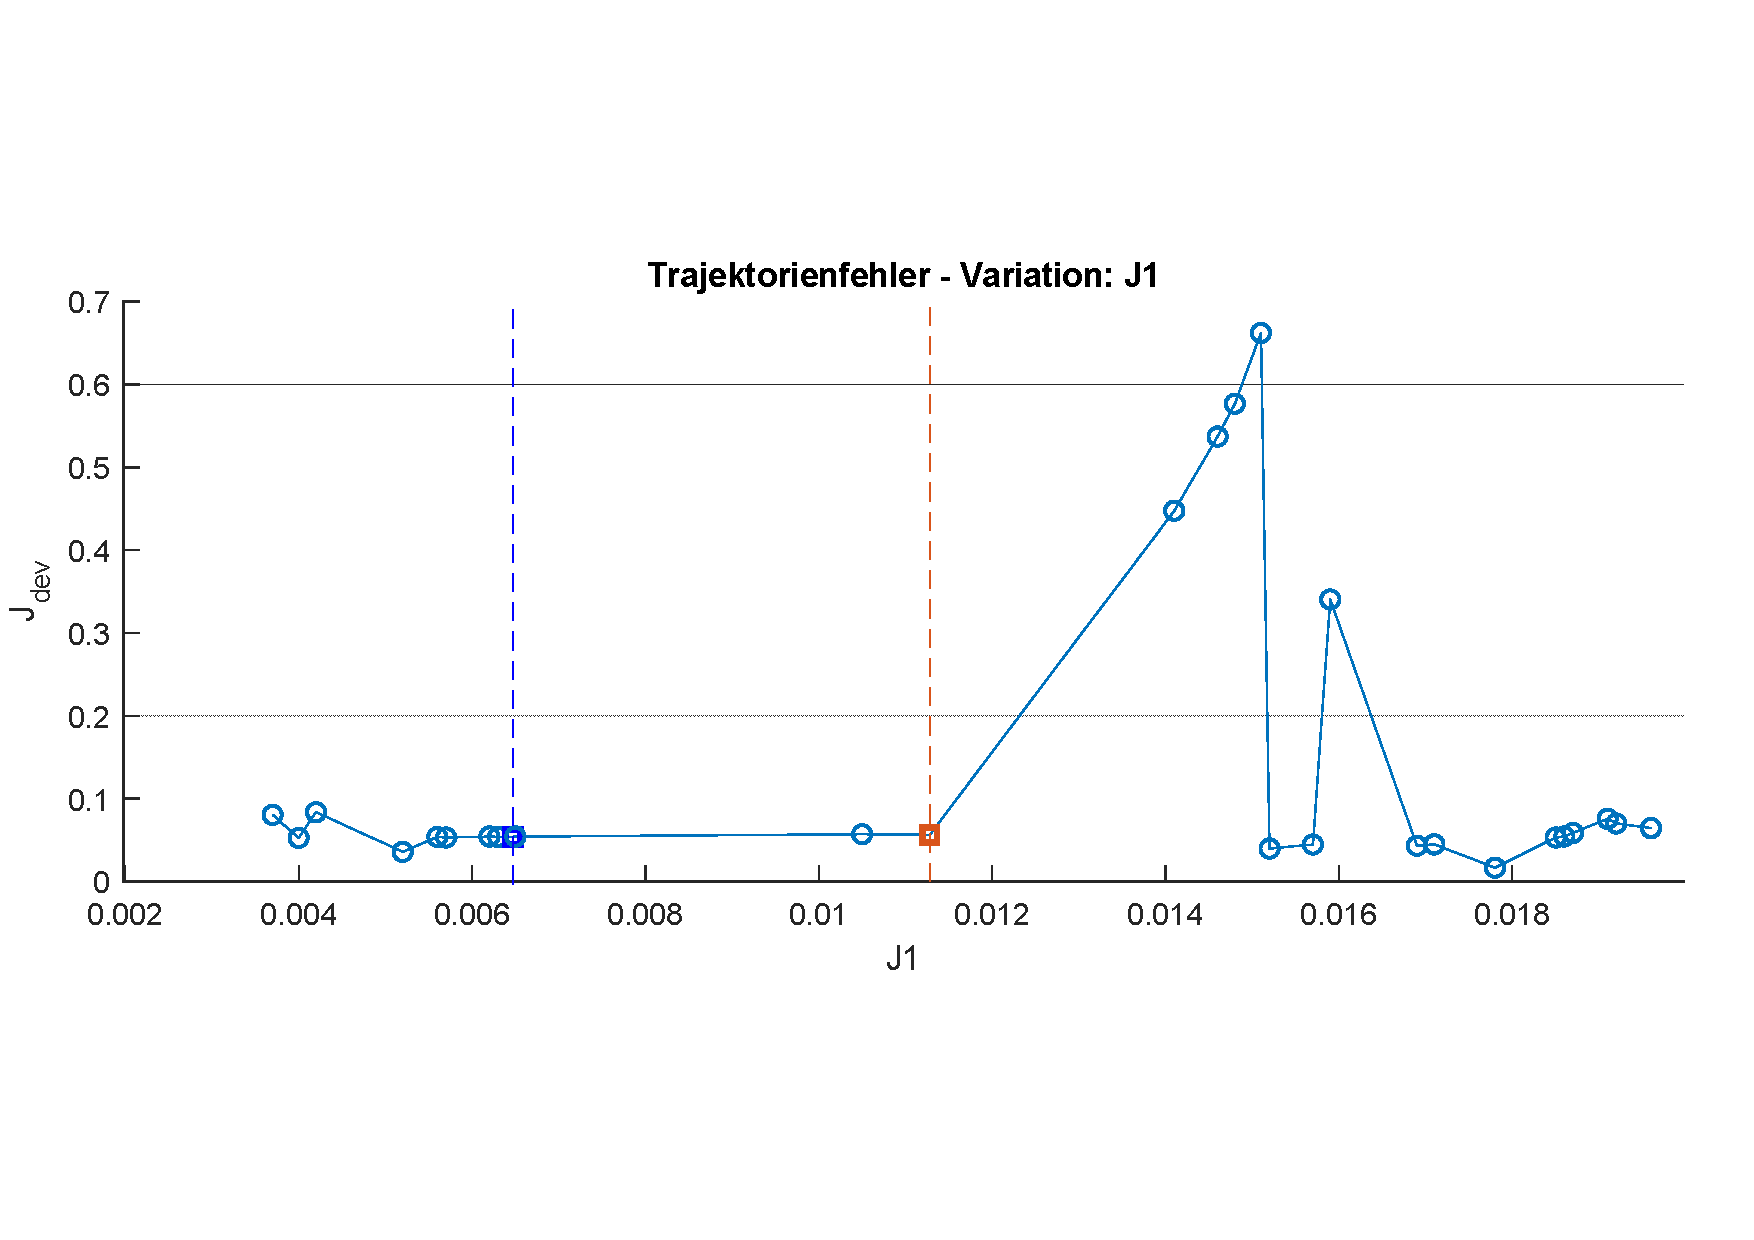
\includegraphics[width=0.8\textwidth]{Bilder/Trajektorien/J1.pdf}
	\caption{Variation $J_1$}
	\label{fig:trjvarJ1}
\end{figure}

Für $J_1$ werden mit insgesamt $\hg=14\%$ nur wenige gültige Trajektorien gefunden. Diese sind über den größten Teil des untersuchten Wertebereichs verteilt. Im Gegensatz zu den anderen Parametervariation wird hierbei auch eine Trajektorie für den Ribeiro-Wert gefunden. Dies lässt sich jedoch nicht mit einem Häufungsbereich weiterer gültiger Trajektorien begründen, wie \figref{fig:trjvarJ1} entnommen werden kann. Häufungen gültiger Trajektorien treten in den gegensätzlichen Bereichen $\valunit{0,0037}{kg m^2}\leq J_1 \leq \valunit{0,0065}{kg m^2}$ mit $\hg=33 \%$ und $\valunit{0,0141}{kg m^2}\leq J_1 \leq \valunit{0,0196}{kg m^2}$ mit $\hg=29 \%$ auf. Es können sich daher sowohl niedrige als hohe Werte für $J_1$ positiv auf die Konvergenz der Trajektorienberechnung auswirken. Der mittlere Bereich hingegen ist hingegen als ungünstig anzusehen, wobei dennoch gültige Lösungen gefunden werden können. Für sehr niedrige Werte existieren wie bei $J_2$ keine gültigen Trajektorien mehr, weshalb wieder eine Untergrenze $J_{2\mrm{min}} = \valunit{0,0037}{kg m^2}$ eingeführt wird.
Trajektorien mit $J_\mrm{dev}>1$ kommen anders als bei $J_2$ nicht vor. Ein erhöhtes Vorkommen von Trajektorien geringerer Güte mit $J_\mrm{dev}>0,1$ wird im Bereich $\valunit{0,0141}{kg m^2}\leq J_1 \leq \valunit{0,0159}{kg m^2}$ beobachtet. Da dieser Bereich wieder einen Grenzbereich einer Häufung gültiger Trajektorien markiert wie bei $m_1$ und $m_2$, könnte dies als Hinweis auf ein Verhaltensmuster der Güte verstanden werden. Die Variationen von $J_2$, $s_1$ und $s_2$ bestätigen diese Interpretation jedoch nicht.  

Mit der definierten Untergrenze wird ein Wertebereich für gültige Trajektorien von $\valunit{0,0037}{kg m^2}\leq J_2 \leq \valunit{0,0196}{kg m^2}$ mit $\Pkon\approx\hg=17 \%$ formuliert.

Aus der Variation der Schwerpunkte $s_1$ und $s_2$ wird kein auffälliges Verhalten identifiziert. Für beide Schwerpunkte können näherungsweise über die gesamte jeweilige Stablänge gültige Lösungen gefunden werden, sodass eine Eingrenzung des Wertebereichs nicht notwendig erscheint. Der Anteil gültiger Trajektorien ist für $s_1$ jedoch deutlich geringer als für $s_2$. Die Trajektorienberechnung reagiert damit prinzipiell empfindlicher auf eine Veränderung von $s_1$. Eine Häufung gültiger Trajektorien tritt wieder im Bereich des Apprich-Wertes auf. Obwohl der Ribeiro-Wert beider Schwerpunkte jeweils in einem solchen Häufungsbereich liegt, wird jeweils keine Trajektorie gefunden. Für die scheinbar ungünstigen Ribeiro-Schwerpunkte ist daher in diesem Fall keine explizite Ursache erkennbar.

Die formulierten Wertebereiche gültiger Trajektorien sind in \tabref{tab:Bereichsempfehlungen} noch einmal abschließend übersichtlich dargestellt. 
\begin{table}[h]
	\centering
	\caption{Wertebereiche gültiger Trajektorien}
		\begin{tabular}{lllll}
			\toprule
			Parameter  & Einfluss & min & max & $\Pkon$ \\
			\midrule
			{$m_1 \ [\unit{kg}]$}  &  hoch & $0$ & $1,07$  & $26 \%$ \\
			%\midrule			
			$m_2 \ [\unit{kg}]$  &  hoch & $0,09$ & $0,39$  & $38 \%$ \\	
			%\midrule
			$J_1 \ [\unit{kg m^2}]$  &  hoch & $0,0037$ & $0,0196$  & $17 \%$ \\
		  %\midrule
			$J_2 \ [\unit{kg m^2}]$ & gering & $0,004$ & $0,02$  & $77 \%$ \\
			%\midrule
			$s_1 \ [\unit{m}]$   &   mittel & $0$ & $0,29$  & $21 \%$ \\
			%\midrule
			$s_2 \ [\unit{m}]$   &   gering & $0$ & $0,338$  & $44 \%$ \\
			\bottomrule
		\end{tabular}
	\label{tab:Bereichsempfehlungen}
\end{table}

Es ist in Bezug auf die Ergebnisse zu berücksichtigen, dass die betrachteten Systemparameter jeweils für sich alleine variiert wurden. Eine Untersuchung bei Variation der Parameter in Abhängigkeit zu einander kann daher von den vorliegenden Ergebnissen abweichen. Ebenfalls sind die vielfältigen Konfigurationsmöglichkeiten der NMPC in Bezug auf die Ergebnisse zu problematisieren. Es ist entsprechend anzunehmen, dass formulierten Wertebereiche bei einer anderen Konfiguration der NMPC mit beispielsweise Variation von Schrittweite, Prädiktionshorizont, Integrator, Gewichtungsmatrizen der Gütefunktion oder anderem Optimierer variieren. Die formulierten Bereichsempfehlungen sind daher nur für die im Rahmen dieser Arbeit definierten Voraussetzungen gültig und in Bezug auf Allgemeingültigkeit in erster Linie als Orientierungshilfen, jedoch nicht als harte Grenzen zu verstehen. 

Die Gültigkeit der ermittelten Bereichsgrenzen muss außerdem für weitere Vergleichstrajektorien überprüft werden und gegebenenfalls trajektorienspezifische Grenzen formuliert werden. 

Die starke Begrenzung der Stabmassen lässt als Ursache eine verstärkte Abhängigkeit von der Stellgrößenbegrenzung vermuten.
Die Stellgrößenreserve bzw. die der NMPC als Nebenbedingung übergebene Kraftbegrenzung birgt somit ein weiteres Variationspotential, wodurch besonders eine Verschiebung der Bereichsobergrenzen zu erwarten ist. 

Die Coulomb-Reibung wurde im Rahmen der Untersuchung vernachlässigt. Erste Tests weisen auf einen erkennbar negativen Einfluss auf die Trajektorienbrechnung hin, was auf die hohe Nichtlinearität zurückgeführt wird. Wie in \secref{subsec:mitInd} werden hierzu verschiedene NMPC-Konfigurationen getestet, wobei lediglich für die Apprich-Parameter inklusive Coulomb-Reibung am Schlitten, exklusive Gelenkreibung, eine akzeptable Trajekorie gefunden wird, ebenfalls wieder für die bekannte NMPC-Konfiguration, die auch für die anderen Parametertests verwendet wurde. Es wird daher für zukünftige Arbeiten empfohlen, die für diese Arbeit gewählte Konfiguration weiterzuverwenden, wenn eine Variation der Reibwerte angestrebt wird.  
